\chapter{\label{ch:analysis}Analysis}
  In this chapter the various parts of the analysis are explained. 
  In Section~\ref{sec:mcSim}, the simulations used to estimate the detector's 
    ability to measure UPC processes are discussed. 
  The selection of UPC events is detailed in Section~\ref{sec:DataSetEvSel}.
  Extraction of the number of coherent \JPsi{} candidates is explained in 
    Section~\ref{sec:sigEx}.
  The determination of the detector's efficiency for measuring UPC events is 
    explained in Section~\ref{sec:effDet}.

  \section{\label{sec:mcSim} Physics generators and Monte Carlo simulations}
    Every physical measurement is the product of the underlying physics 
      folded with the response of the detector used to do the measurement. 
    In order to understand the underlying physical process, the detector's 
      effect on the measurement must be understood and accounted for. 
    As instruments become more and more complicated, the interplay among all
      of the many parts of the detector makes an analytic approach to the 
      problem untenable.
    For this reason, the numerical technique of Monte Carlo (MC) simulation is
      often the most effective approach for describing detector effects.

    MC simulations use random number generation to model the many statistical 
      effects of particles interacting with different parts of the detector. 
    First, particles are generated according to theoretical distributions.
    These particles are then propagated through a simulation of the detector.
    As the particles pass through the detector, random numbers are used
      to determine how these particles interact with the materials of the 
      detector based on the known properties of the material. 
    In this way, the theoretical distributions are convolved with a realistic 
      model of the detector's response. 
    A more detailed picture of how the detector shapes the underlaying 
      distributions emerges with each successive event.
    The final goal of the MC simulation is to produce a set of events that 
      accurately reproduce what would be measured if the theoretical input 
      describes nature well. 

  \subsection{STARlight and particle gun MC}
    In this thesis, two classes of generator input samples were used, 
      STARlight \cite{vmd1999, starlight} and a particle gun.
    The STARlight samples correspond to the theoretical calculations 
      described in Section~\ref{sec:vdmTheory}, while the particle gun produces
      particles with a user defined transverse momentum distribution and 
      rapidity distribution and isotropic decay to muon pairs in the \JPsi{} 
      rest frame. 
    For STARlight, three different physical processes were simulated:
      coherent \JPsi{} production, where the photon couples to the nucleus as
      a whole; incoherent \JPsi{} production; where the photon couples to a
      single nucleon within the nucleus, and photon-photon interactions, where 
      the photons from the two nuclei interact with each other to produce a 
      pair of oppositely charge muons.
    All three STARlight samples contain a $\mu^{+}$ and $\mu^{-}$ in the final 
      state.

    Because STARlight is not integrated into the standard CMS software 
      framework (CMSSW), a simulation software chain with 5 steps 
      was developed.
    First, STARlight is run in the specified mode, and a single file is 
      created for each physics process. 
    In step 2, the STARlight output file is converted to the Les Houches Event 
      (LHE) format \cite{lheFormat}, and the momentum of the parent \JPsi{} or 
      the initial photon-photon pair is added to the record of each event.
    The event record produced by STARlight only contains the final state 
      particles.
    To process the events in parallel, the STARlight files are subdivided 
      in step 2, creating several LHE files from a single STARlight file.
    The LHE files are used as input to CMSSW.

    Steps 3 to 5 take place within CMSSW. 
    In step three the generated particles are propagated through the GEANT4 
      \cite{geant} detector simulation.
    This accounts for all the interactions with the detector and produces as 
      output a format identical to the raw data that is recorded during data
      taking.
    Steps 4 and 5 are processed using the same software as in data taking.
    In step 4 the reconstruction software used during data taking is run on 
      the output of the detector simulation.
    The output of the reconstruction is reduced to the information that is 
      needed for the final analysis in the final step.

    The particle gun samples were created entirely within CMSSW.
    \JPsi{} mesons were created according to user defined \pt{} and rapidity
      distributions. 
    The decay of \JPsi{}s to a $\mu^{+}$$\mu^{-}$ pair was simulated with
      a uniform decay distribution, corresponding to unpolarized \JPsi{} 
      particles.
    As with the STARlight samples, these muons are propagated through the GEANT4
      simulation \cite{geant} of the detector, and the raw data is produced.
    The remaining steps of running the reconstruction code and reducing the 
      data to the final data format needed for the analysis are identical to 
      the STARlight production.

    The momentum of the final state muons is the main driver of whether the 
      candidate can be measured.
    One of the two daughter muons must have large enough momentum to fire the 
      trigger, and both muons must have enough momentum to be 
      reconstructed and tagged as a muon. 
    There are at least 10 interaction lengths of material through which the 
      muons must travel in order reach the muon chambers 
      (see Fig.~\ref{fig:matThick}).
    This imposes an effective momentum threshold of about 7 GeV in order for 
      muons can fire the trigger. 

    The \pt{} distribution and the polarization of the \JPsi{}s produced are 
      the main factors controlling the momentum of the muon daughters, which
      vary for the different MC samples. 
    The polarization effects how the momentum is shared between the daughters
      \cite{oniaPol}.
    In the rest frame of the parent \JPsi{}, equal momentum is given to each 
      daughter muon. 
    However in the lab frame of the detector, the muon daughters which are 
      emitted from transversely polarized \JPsi{} will tend to be emitted in
      the direction the \JPsi{} is traveling and will have unequal momenta.
    The daughter traveling in the direction of the \JPsi{} will have increased
      momentum, whereas the daughter traveling opposite to the \JPsi{} 
      direction will have decreased momentum. 

    In Fig.~\ref{fig:starlightRapPtDist} the \JPsi{}s \pt{} from the 
      STARlight generated coherent, and incoherent, and the dimuon \pt{} for 
      photon-photon samples are compared.
    Both the coherent and the photon-photon samples are concentrated at low 
      \pt{}, and neither sample extends much beyond 0.15 GeV.
    The incoherent sample is peaked near 0.5 GeV and extends beyond 1 GeV.
    The two particle gun samples resemble the incoherent and coherent samples
      \pt{} distributions.
    The first sample has a Gaussian \pt{} distribution extending to 
      approximately 0.15 GeV, whereas the second is flat in \pt{} up to
      2 GeV.
    \begin{figure}[!Hhbt]
      \centering
      $ \begin{array}{cc}
        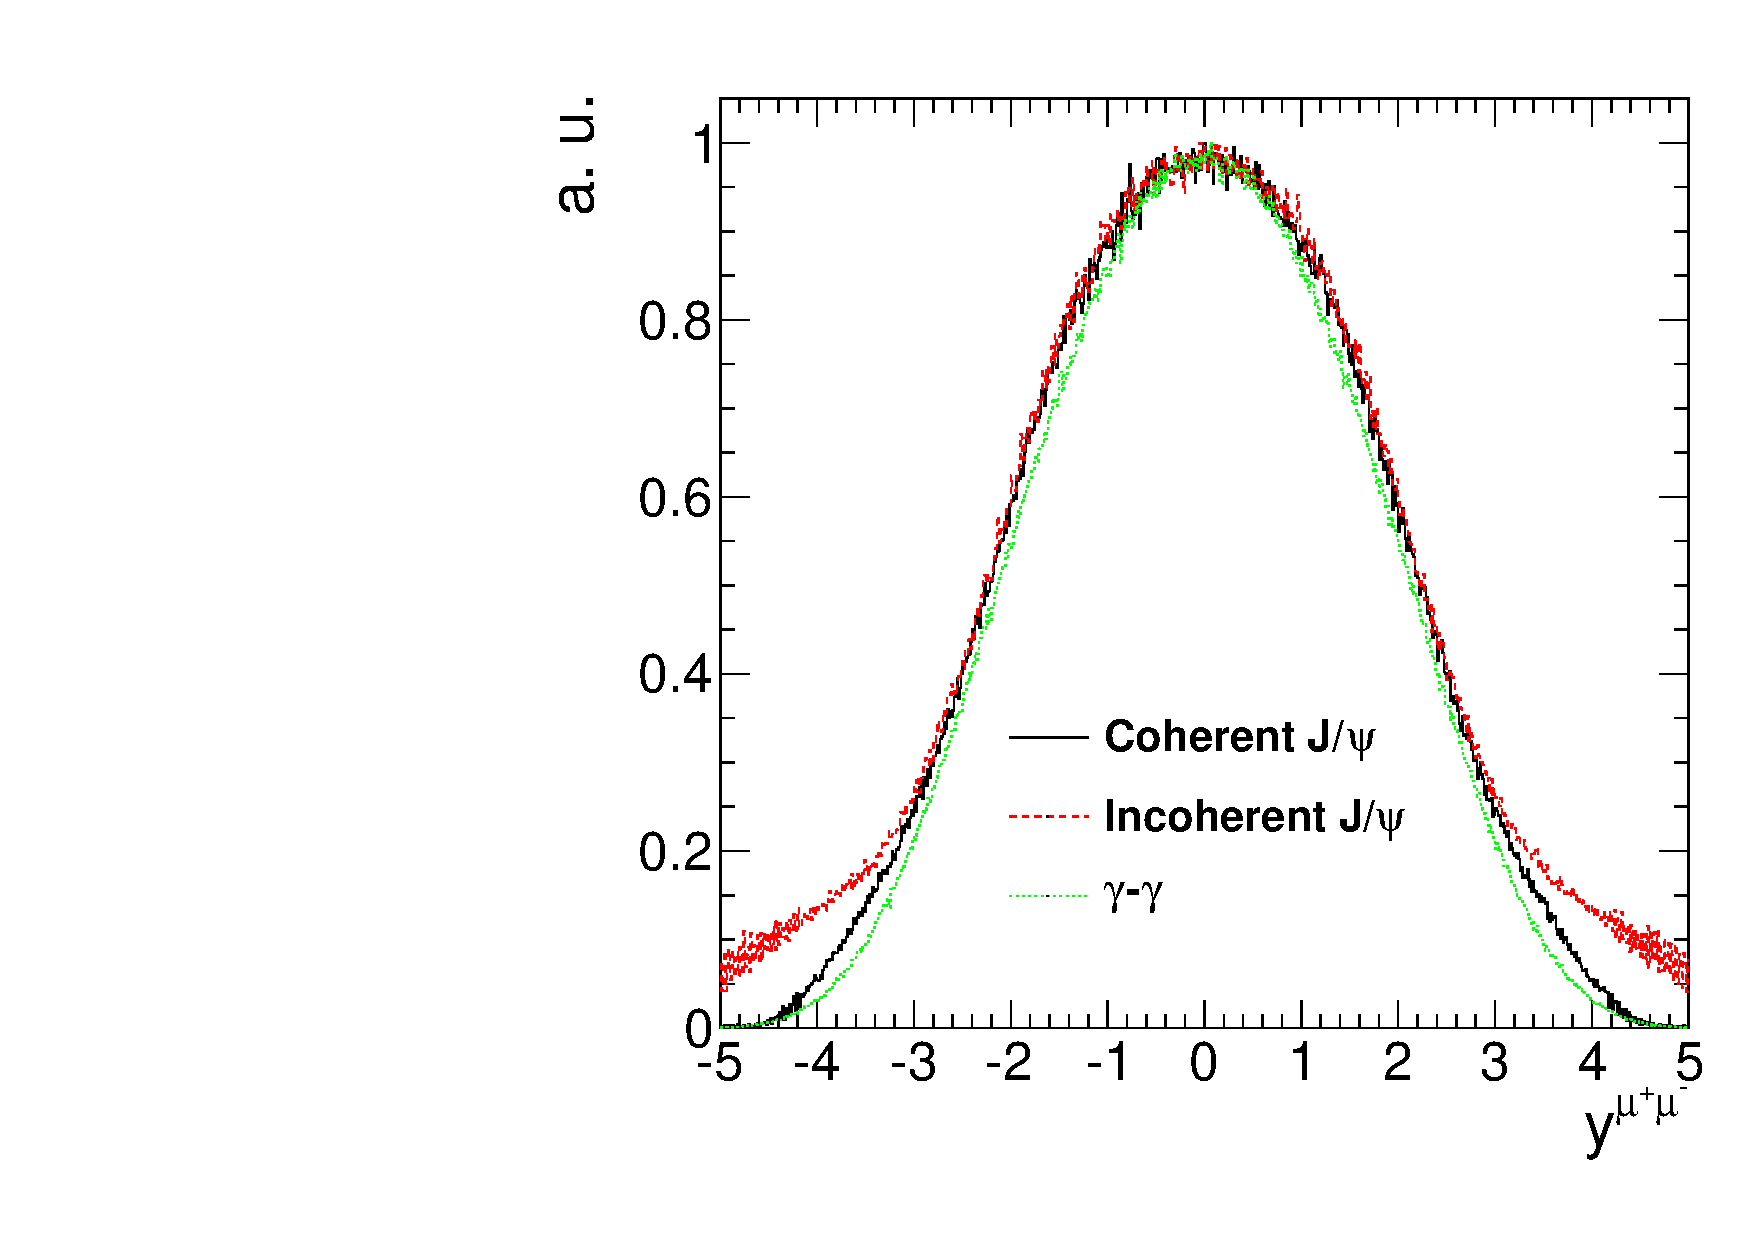
\includegraphics[width=0.45\textwidth]{genRapDis} &
        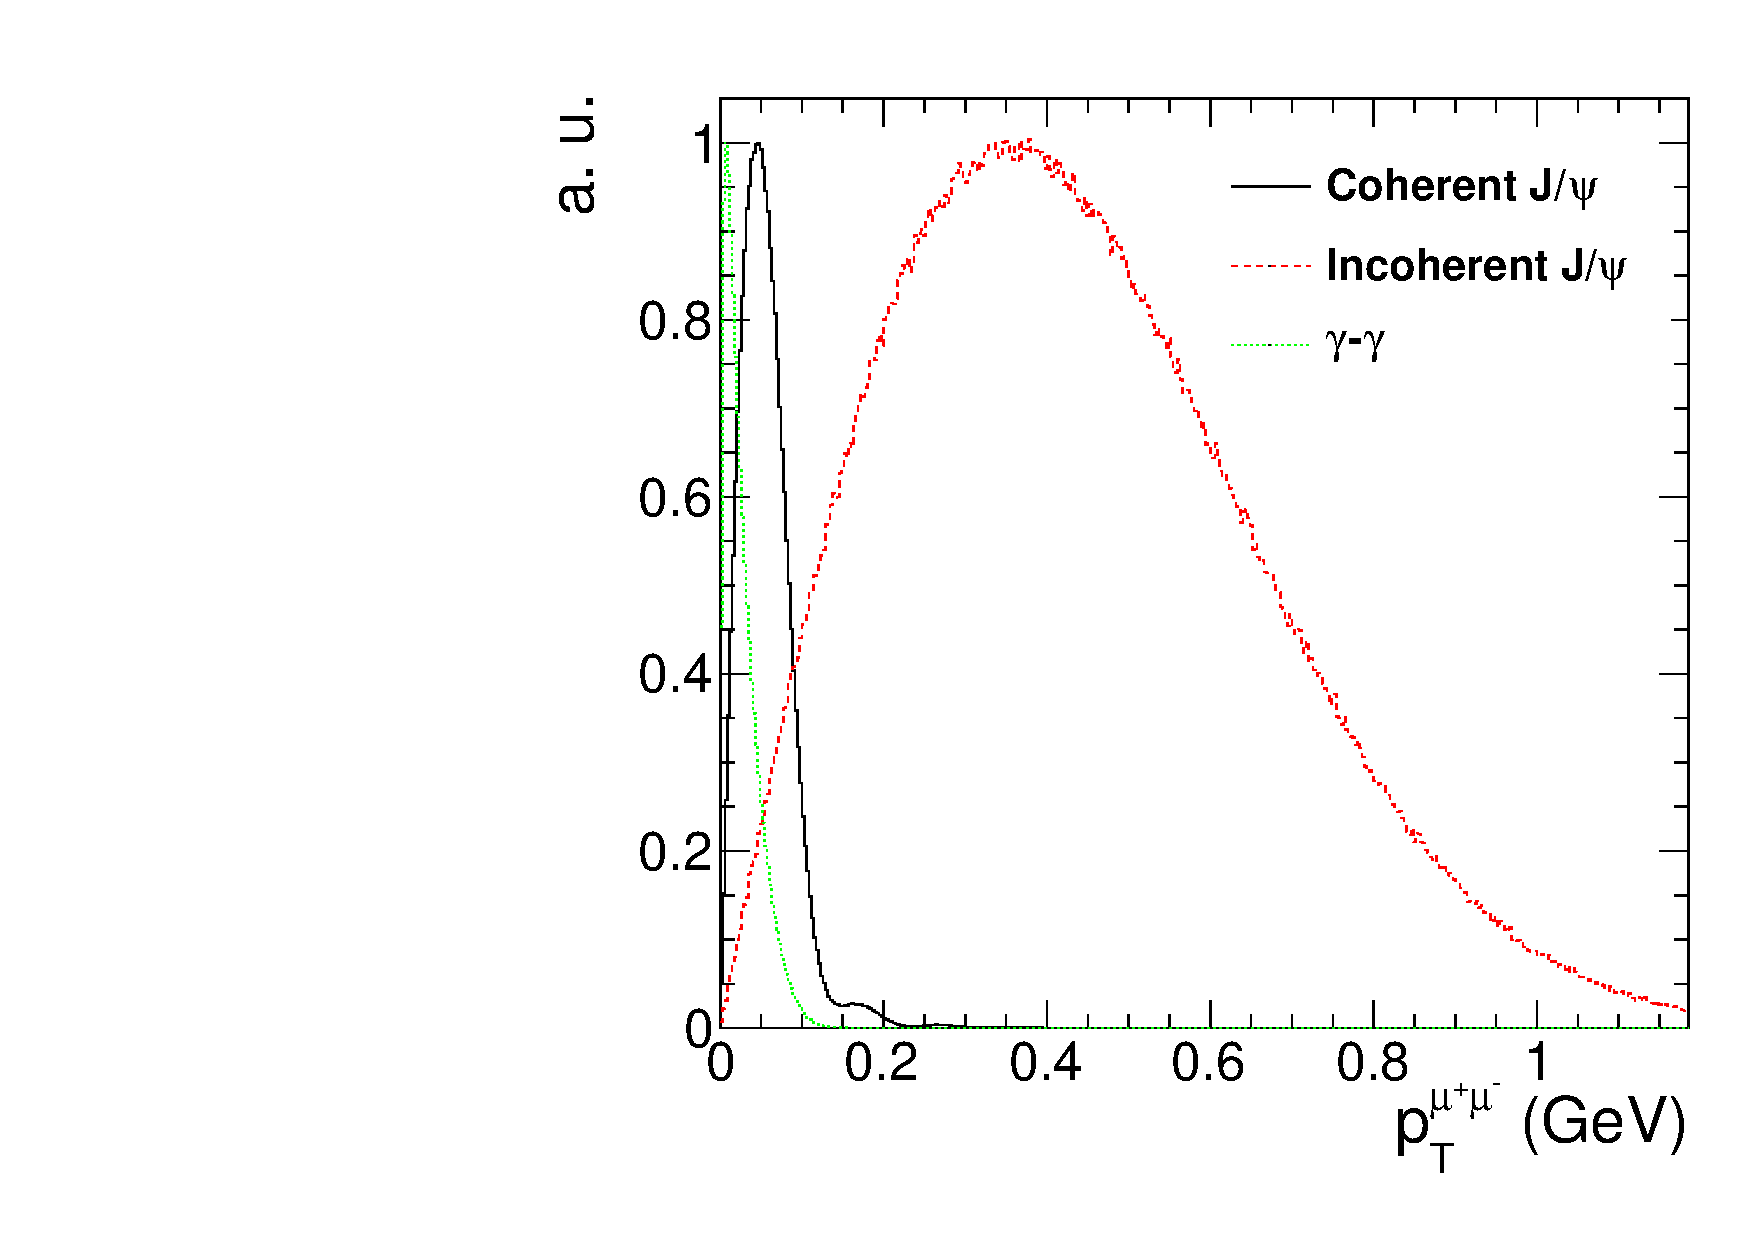
\includegraphics[width=0.45\textwidth]{genPtDis}
      \end{array} $
      \caption{Generator level rapidity (left) and \pt{} (right) 
          distributions for the coherent (black), incoherent (red), 
          and photon-photon process (green).}
      \label{fig:starlightRapPtDist}
    \end{figure}
    
    The particle gun samples are unpolarized, whereas the STARlight samples 
      have transverse polarization.
    The cosine of the helicity angle, the angle between the \JPsi{} spin vector
      in the rest frame and the direction of the boost to the lab frame, are 
      shown for the particle gun samples and the STARlight samples in 
      Fig.~\ref{fig:genHXAngle}. 
    For the STARlight sample the helicity angle prefers to be either parallel or
      anti-parallel.
    However, the particle gun samples have no preferred direction.
    \begin{figure}[!Hhbt]
      \centering
      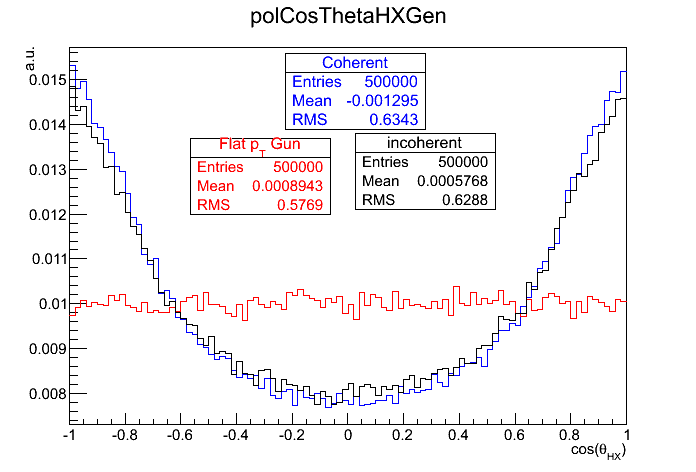
\includegraphics[width=.6\textwidth]{polCosThetaHXGen}
      \caption{ The \JPsi{} polarization of the particle gun (red),
        coherent (blue), and incoherent samples are plotted as the
        cosine of the helicity angle.} 
      \label{fig:genHXAngle}
    \end{figure}

      \begin{figure}[!Hhbt]
        \centering
        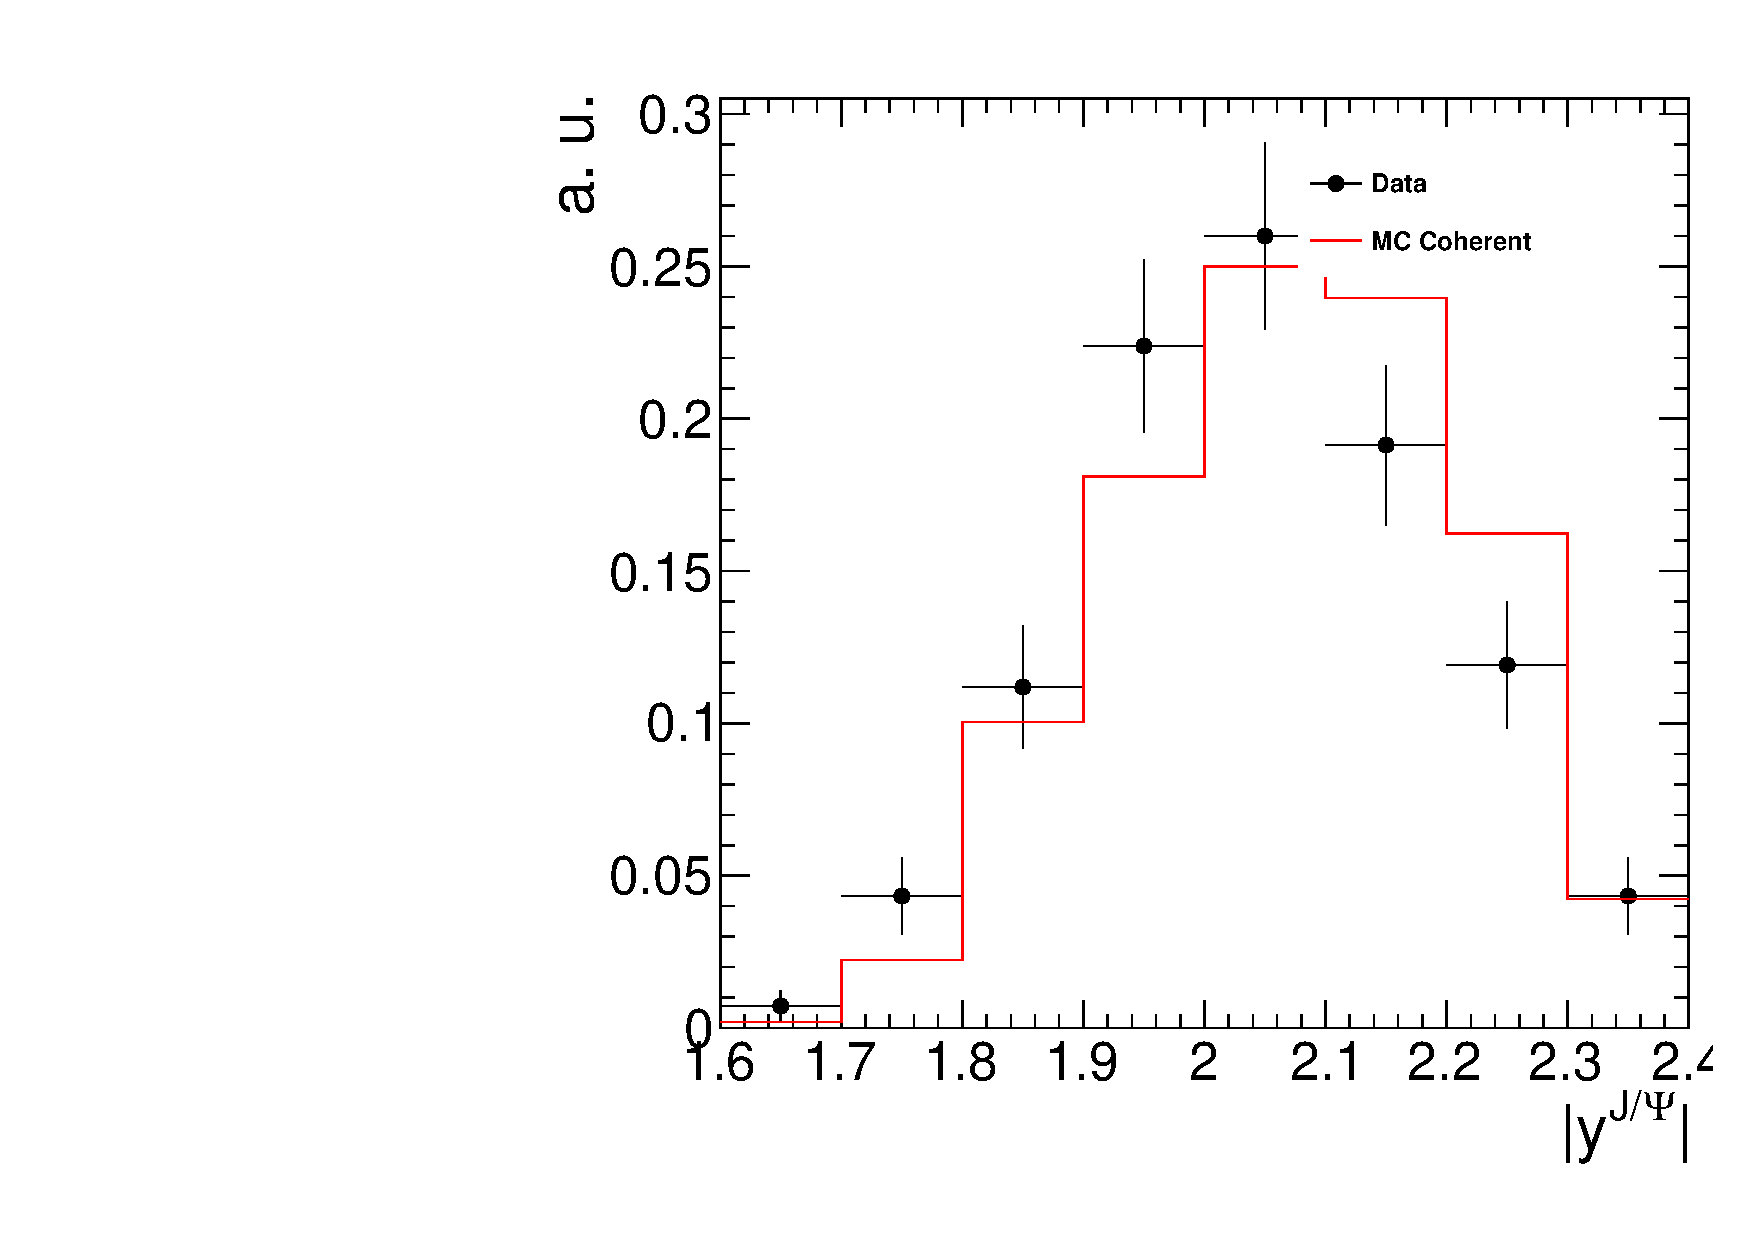
\includegraphics[width=0.5\textwidth]{jpsiMcComp/jpsiAbsRapCoherent}
        \caption{Comparison of the of the dimuon rapidity distributions between 
          coherent \JPsi{} MC sample and data.}
        \label{fig:jpsiAbsRapCoherent}
      \end{figure}
      \begin{figure}[!Hhbt]
        \centering
        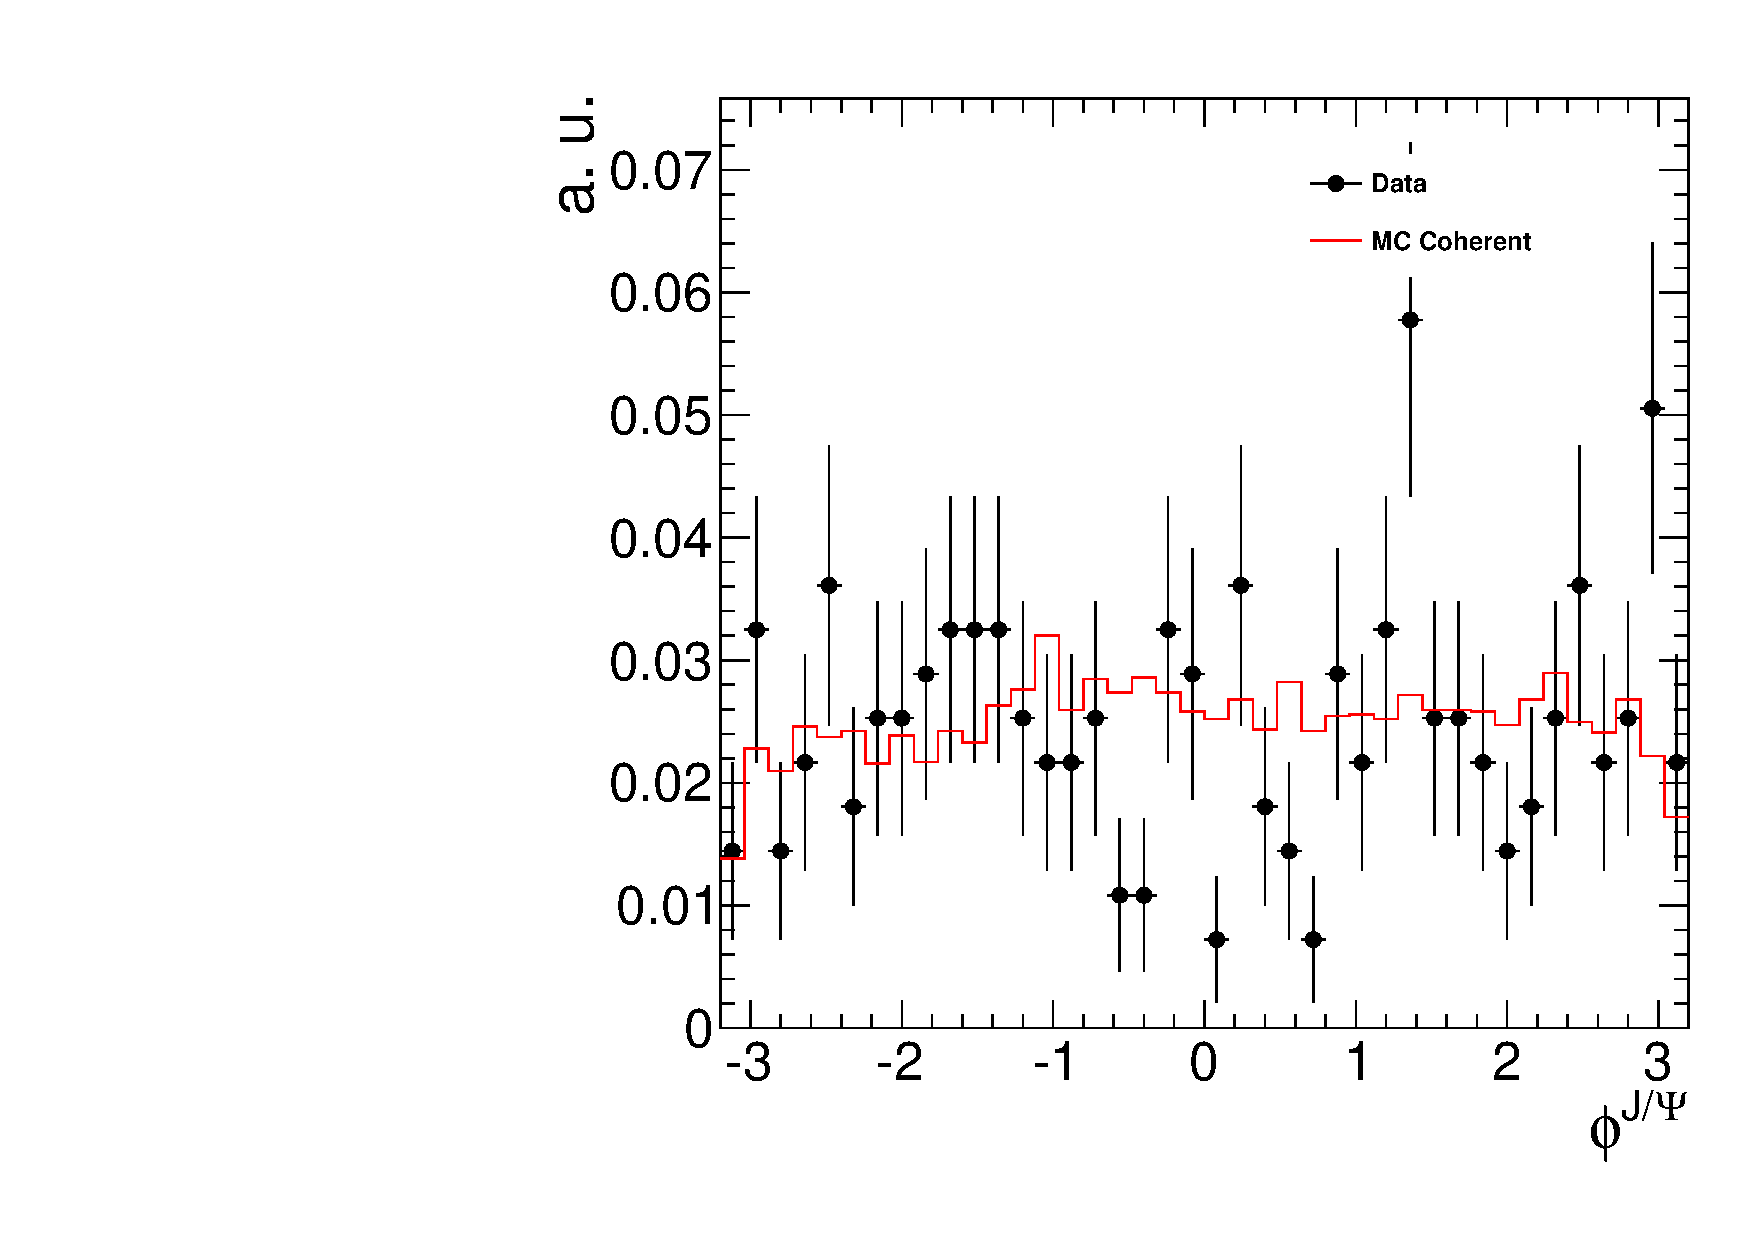
\includegraphics[width=0.5\textwidth]{jpsiMcComp/jpsiPhiCoherent}
        \caption{Comparison of the of the dimuon $\varphi$ distributions 
          between coherent \JPsi{} MC sample and data.}
        \label{fig:jpsiPhiCoherent}
      \end{figure}
      \begin{figure}[!Hhbt]
        \centering
        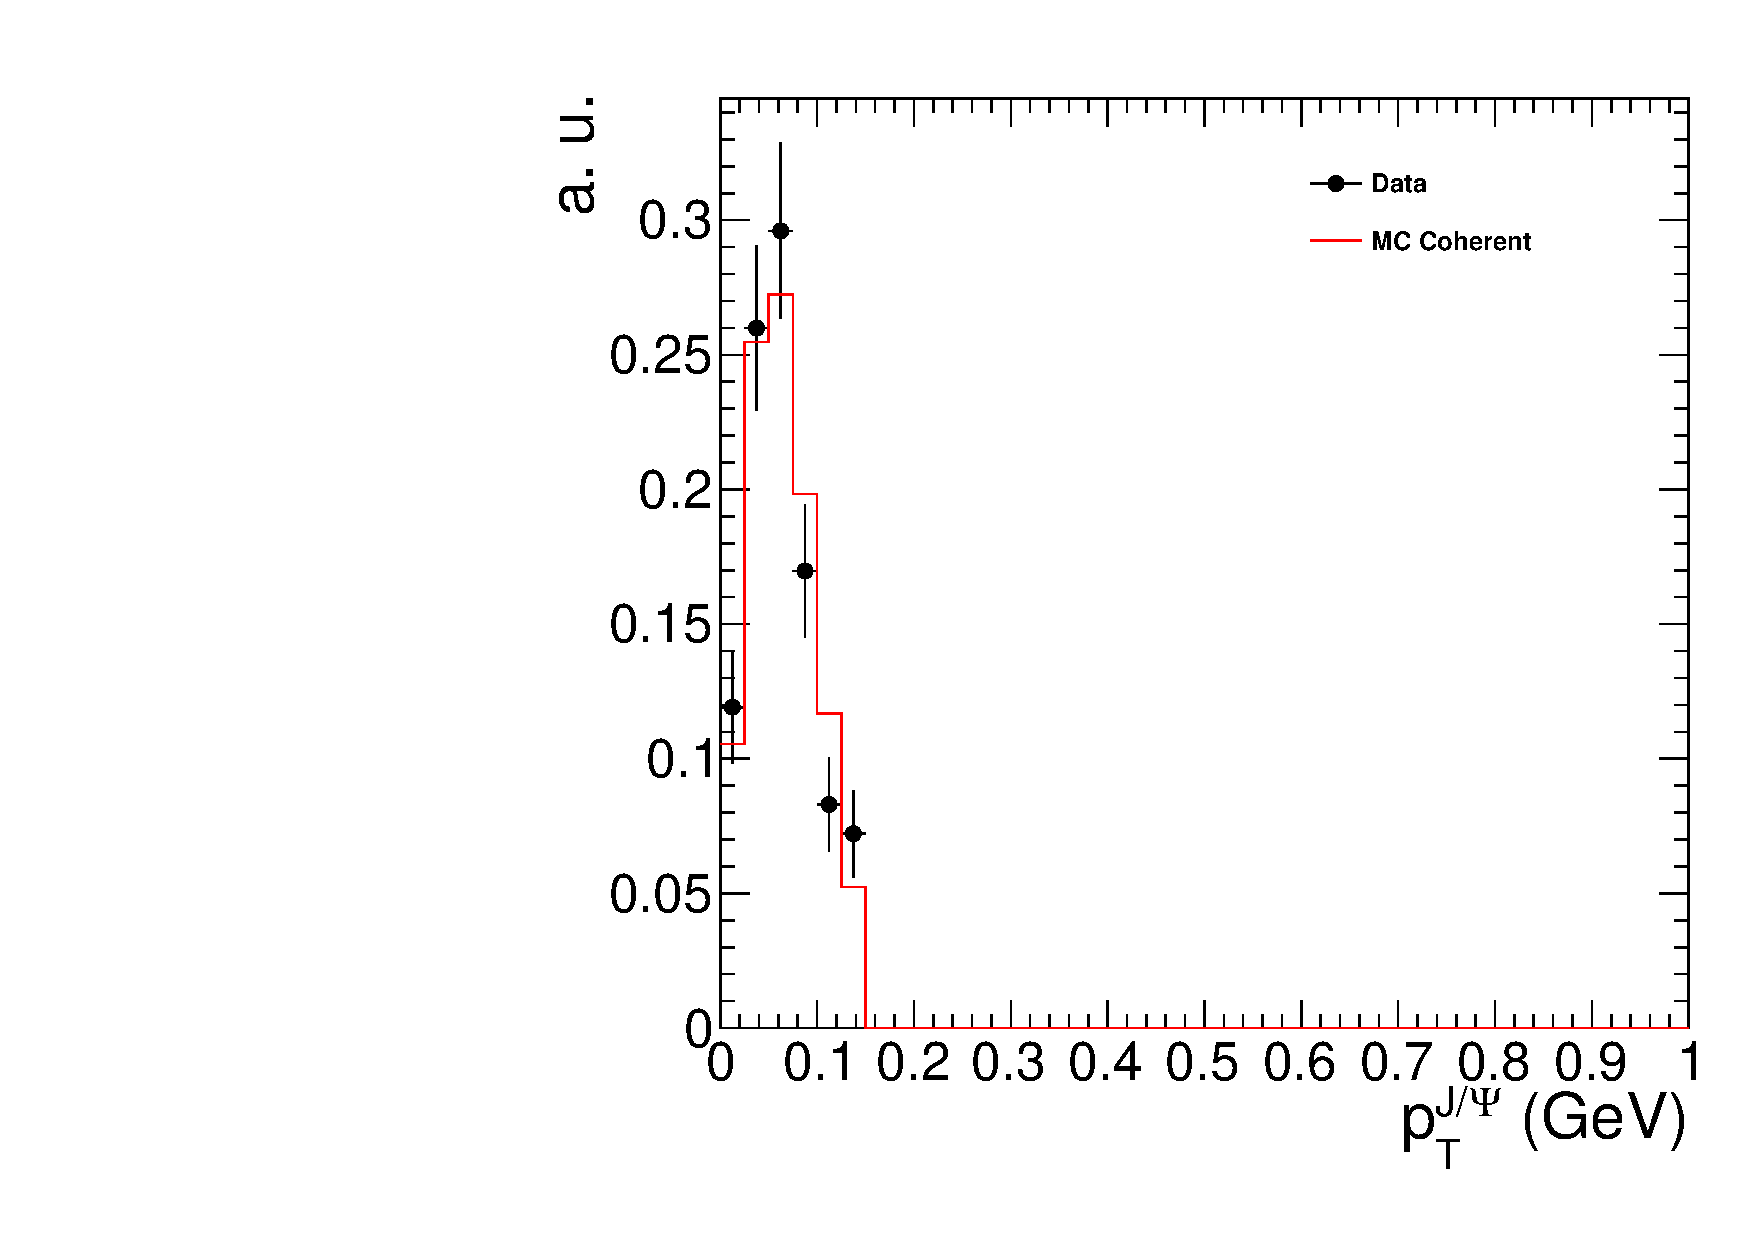
\includegraphics[width=0.5\textwidth]{jpsiMcComp/jpsiPtCoherent}
        \caption{Comparison of the of the dimuon \pt{} distributions 
          between coherent \JPsi{} MC sample and data.}
        \label{fig:jpsiPtCoherent}
      \end{figure}
    Figures \ref{fig:jpsiAbsRapCoherent}, \ref{fig:jpsiPhiCoherent}, and
      \ref{fig:jpsiPtCoherent} show  the rapidity, $\phi$, and  \pt{} 
      distributions of reconstructed coherent \JPsi{} from STARLight MC and 
      data. 
    All distributions are normalized to one. 
    The mean of the STARLight rapidity distribution is slightly shift by 
      $\approx 0.1$ to higher rapidity. 
    The $\phi$, and  \pt{} distributions from STARLight and data are both
      very similar. 

  \section{\label{sec:DataSetEvSel} Event selection}
    The unprecedented amounts of data produced by the LHC has made it possible 
      to investigate novel physics processes like UPC \JPsi{} production.
    The data for this analysis were recorded during the 2011 LHC PbPb run. 
    During this period, 150 $\mu$$b^{-1}$ were recorded by the CMS detector,
      corresponding to > 10$^{9}$ PbPb collisions. 
    Of this, 143 $\pm$ 7 (syst) $\mu$$b^{-1}$ of data were used in this analysis due to the 
      ZDCs being temporally disconnected to test the Forward Shower Counters.
  
    \subsection{Data sets}
      The data were dived into three specially selected samples, Physics, Monitoring, 
        and Zero bias, based on the triggers which recorded the events (see 
        Table~\ref{tab:sampleLumiNevt}).
      By recording this hierarchy of samples, interesting events are selected 
        with a much higher purity in the physics sample, while the zero bias 
        and ZDC triggered samples allow for the investigation of the selection 
        criteria. 
      The purity, which is a measure of how many signal events relative to
        background events are in a sample, is obtained by using more selective
        triggers.
      Less selective triggers, those assigned to the monitoring and zero bias 
        samples, were used to investigate to what extent signal events are lost
        because of the higher selectivity of physics triggers. 
      These samples were recorded using subsets of the HLT triggers found in 
        Table~\ref{tab:hltTriggers2011} of Chapter~\ref{ch:trigg}.
      The \JPsi{} events discussed in this thesis were obtained by analyzing 
        the sample labeled in Table~\ref{tab:sampleLumiNevt} as physics.
      A ZDC triggered monitoring sample was recorded for the sake of estimating
        efficiencies.
      Lastly, a zero bias sample was recorded for investigating the ZDC and the 
        noise distributions of HF.
  
      The physics sample containing the \JPsi{} signal was recorded by the muon 
        trigger labeled ``L1UPCMuon and Pixel Track'' in 
        Table~\ref{tab:hltTriggers2011}. 
      Because of the characteristically low momentum of UPC \JPsi{} as compared
        to \JPsi{} created by other physics processes, the loosest muon 
        trigger was used.
      The noise trigger rate for the muon trigger alone was 50 Hz, but in 
        coincidence with the BCS veto and the ZDC trigger the noise rate was
        below 2 Hz. 
      By pairing the muon trigger with the ZDC on the L1 trigger, the noise contribution
        was reduced from the noise contribution from either of the two 
        sub-detectors to the noise coincidence between the two sub-detectors. 
      Contributions from hadronic interactions were reduced by the veto on the 
        BSCs.
      This trigger was designed to balance reducing the rate with maximizing 
        the efficiency, allowing for the data to be recorded without 
        producing high rates that would have resulted in dead time for the 
        detector.  
      
      In order to investigate the muon trigger and the other parts of the event 
        selection, a monitoring sample was recorded by requiring energy 
        consistent with at least one neutron in either of the ZDCs.
      Neutron production is a much more common process than the UPC \JPsi{} 
        production.
      This process has cross sections on the order of 200 b compared
        to 10 mb predicted for \JPsi{} production. 
      For this reason, the rates of this trigger are much higher than the physics
        trigger, and only a small sub set of these events are recorded.
      From this trigger the pixel track portion of the HLT trigger efficiency 
        was estimated as well as the ZDC trigger efficiency, as will be described 
        in Section~\ref{sec:effDet}. 
  
      In addition to the monitoring and physics sample, a zero bias sample was 
        recorded to examine the ZDC neutron reconstruction and the HF noise 
        distributions. 
      The zero bias trigger fired every time both beams passed through CMS. 
      Only 4 events out of every million triggered were recorded for this sample. 
      This sample allowed for an unbiased measurement of the ZDC neutron 
        threshold energies as discussed in Section~\ref{sec:breakUpDet}. 
      Because the zero bias trigger only requires the presence of both LHC 
        beams, the sample contains very few hadronic collisions. 
      This allowed for a measurement of the electronic noise distribution of
        the HF detector, which is important to reducing contamination from 
        hadronic interactions.
  
      The integrated luminosity for each of the three samples is calculated
        by recording activity in HF \cite{cmsLumi}. 
      The cross section for HF activity is measured from a van der Meer scan 
        \cite{vanderMeer:1968zz}. 
      In this way, the amount of integrated luminosity for any running period is
        related to the activity in HF. 
      \begin{table}
  	    \centering
  	    \begin{tabular}{|l|l|l|}
  	      \hline Sample & Events & $\mathcal{L}_{int}$ \\ \hline \hline
          Physics & 346K & 143.3 $\mu$$b^{-1}$ \\ \hline
          Monitor & 1.1M & 31.6 $mb^{-1}$ \\ \hline
          Zero Bias & 8.8M & 580 $b^{-1}$ \\ \hline 
  	    \end{tabular}
  	    \caption{Integrated luminosities and number of events for the three
  	      samples used in this analysis.}
  	    \label{tab:sampleLumiNevt}
      \end{table}
  
    \subsection{Event selection cuts}
      The analysis described in this thesis focuses on UPC \JPsi{}s decaying to 
        muons. 
      The trigger used for this analysis recorded 346841 events.
      A set of off-line cuts was applied to increase the relative contribution 
        of UPC events to background processes. 
      Two sets of event selection cuts were applied to reject background events. 
      The first set rejects background from the beam.
      The second rejects events where hadronic collisions have occurred.
      Table~\ref{tab:evSelCutNumbers} summarizes all the event selection cuts.
      Figure~\ref{fig:evDisplay} shows a candidate event after applying all 
        event selection cuts. 
      \begin{table}[!Hhbt]
        \centering
        \begin{tabular}{|c|c|c|} \hline 
          Cut type & Cut & Events \\ \hline
          -- & all triggered & 346841 \\ \hline
          \multirow{3}{*}{beam background rejection} & good vertex requirement & 340997 \\ \hhline{~--}
          & beam halo muon rejection & 302777 \\ \hhline{~--}
          & cluster shape compatibility requirement & 233590 \\ \hline
          \multirow{3}{*}{hadronic interaction rejection} & single-sided neutron requirement & 149992 \\ \hhline{~--}
          & two track requirement & 32732 \\ \hhline{~--}
          & HF signal rejection & 5392 \\ \hline
          fake muon rejection & muon quality requirement & 2047 \\ \hline
          \multirow{2}{*}{kinematic cut} & \JPsi{} mass requirement & 696 \\ \hhline{~--}
          & muon detectability cuts & 567 \\ \hline
        \end{tabular}
        \caption{Effects of event selection cuts.}
        \label{tab:evSelCutNumbers}
      \end{table}
      \begin{figure*}[!Hhbt]
        \centering
        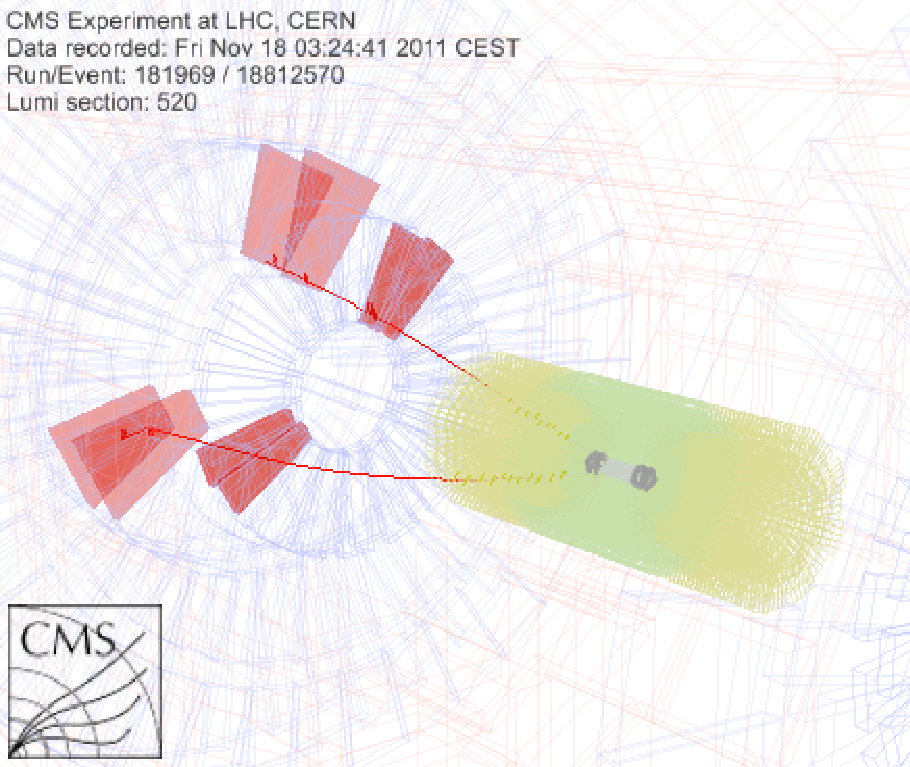
\includegraphics[width=.45\textwidth]{3dRecHitWhite}
        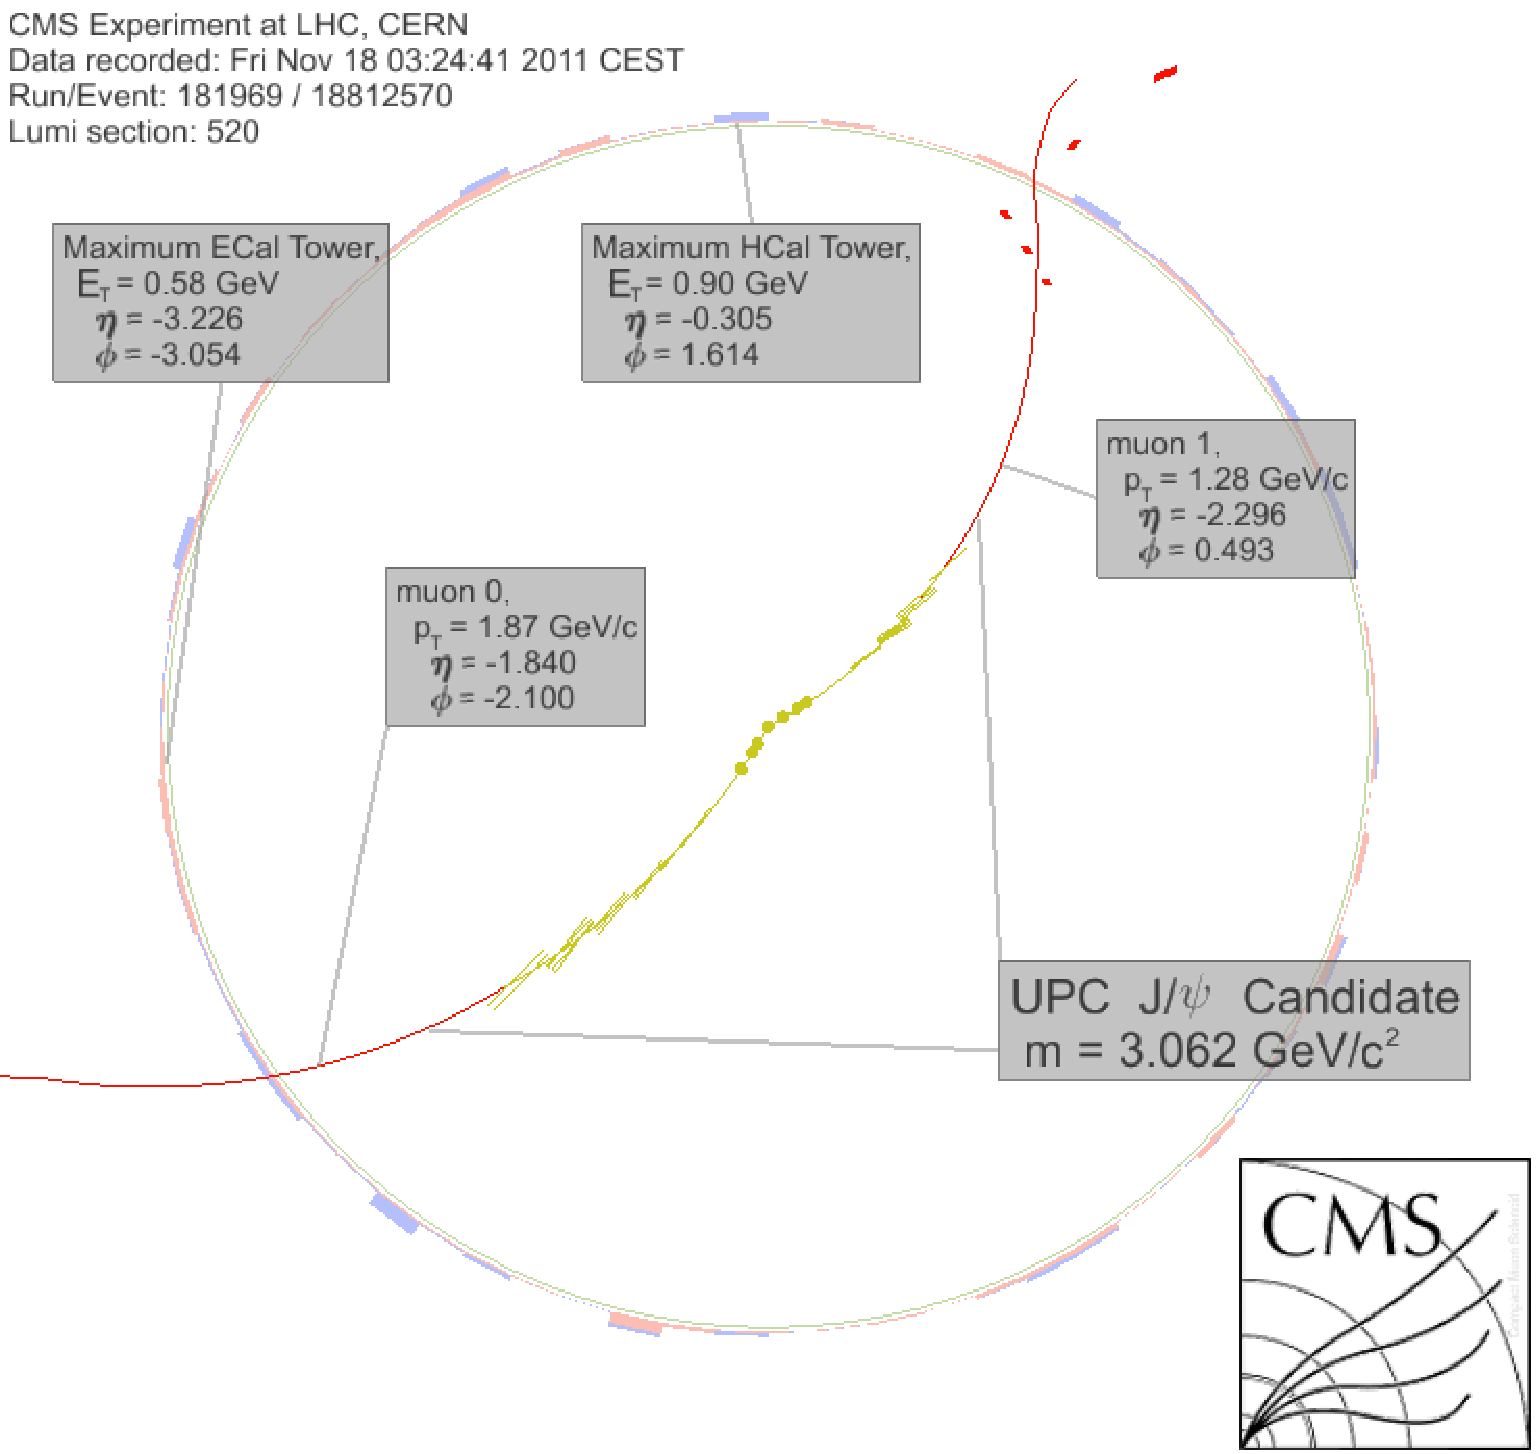
\includegraphics[width=.45\textwidth]{phiRhoWhite}
        \caption{Event display of a UPC \JPsi{} candidate event.}
      \label{fig:evDisplay}
      \end{figure*}
      
      To reject beam induced background the following cuts were applied:
      \begin{itemize}
        \item The reconstructed vertex must be within 2 cm in 
          the transverse direction and 25 cm in the 
          longitudinal direction. This cut ensures that reconstructed particles 
          come from interactions between the two beams rather than event where 
          one of the two beams interact with gas particles near the interaction 
          point. 
  	    \item Beam halo muons were rejected using the timing of the muon hits.
          The beam halo cut rejects events where muons surrounding the beam 
          stream through the detector. 
  	    \item Pixel cluster shape should be compatible with the vertex. 
          This cut requires that energy deposited in the silicon tracker have a
            shape consistant with the primary vertex. 
      \end{itemize}
      When applied after all other cuts these beam background cuts do not reject
        any UPC \JPsi{} candidates. 
  
      The second set of background rejection cuts were designed to 
        reduce contamination from hadronic interactions. 
      \begin{itemize}
  	    \item No more than 2 reconstructed tracks in the event.
  	    \item Maximum reconstructed hit energy in HF was required to be below 
            the threshold for electronic noise. 
          Nearly all hadronic interactions (about 98\%) produce particles in 
            the range $3<|\eta|<5$ covered by the HF detector.
          By requiring that the energy deposits in HF resemble noise, nearly all
            inelastic hadronic collisions are expected to be rejected.
  	    \item Energy in the ZDCs consistent with neutrons on only one side 
            of the interaction point.
          In hadronic interactions both nuclei break-up. 
          By requiring that ZDC only reconstruct neutrons on one side of the 
            interaction point, hadronic interactions that produce neutrons on 
            both sides were rejected.
      \end{itemize}
      Each of these cuts were designed to reject topologies produced by 
        hadronic interactions.
      The effect of these cuts can be seen in Table~\ref{tab:evSelCutNumbers} 
        and are denoted hadronic interaction rejection. 

      To establish the HF noise thresholds, the noise distributions were 
        measured in zero bias events. 
      An offline selection of events with no reconstructed tracks was used
        to ensure that no collision had taken place. 
      The HF noise threshold was defined as the cut that keeps 99\% of the 
        zero bias events.
      The noise distribution from this zero bias sample is compared to the 
        physics sample and MC in Fig.~\ref{fig:hfNoiseDist}.

      \begin{figure}[!Hhbt]
        \centering
        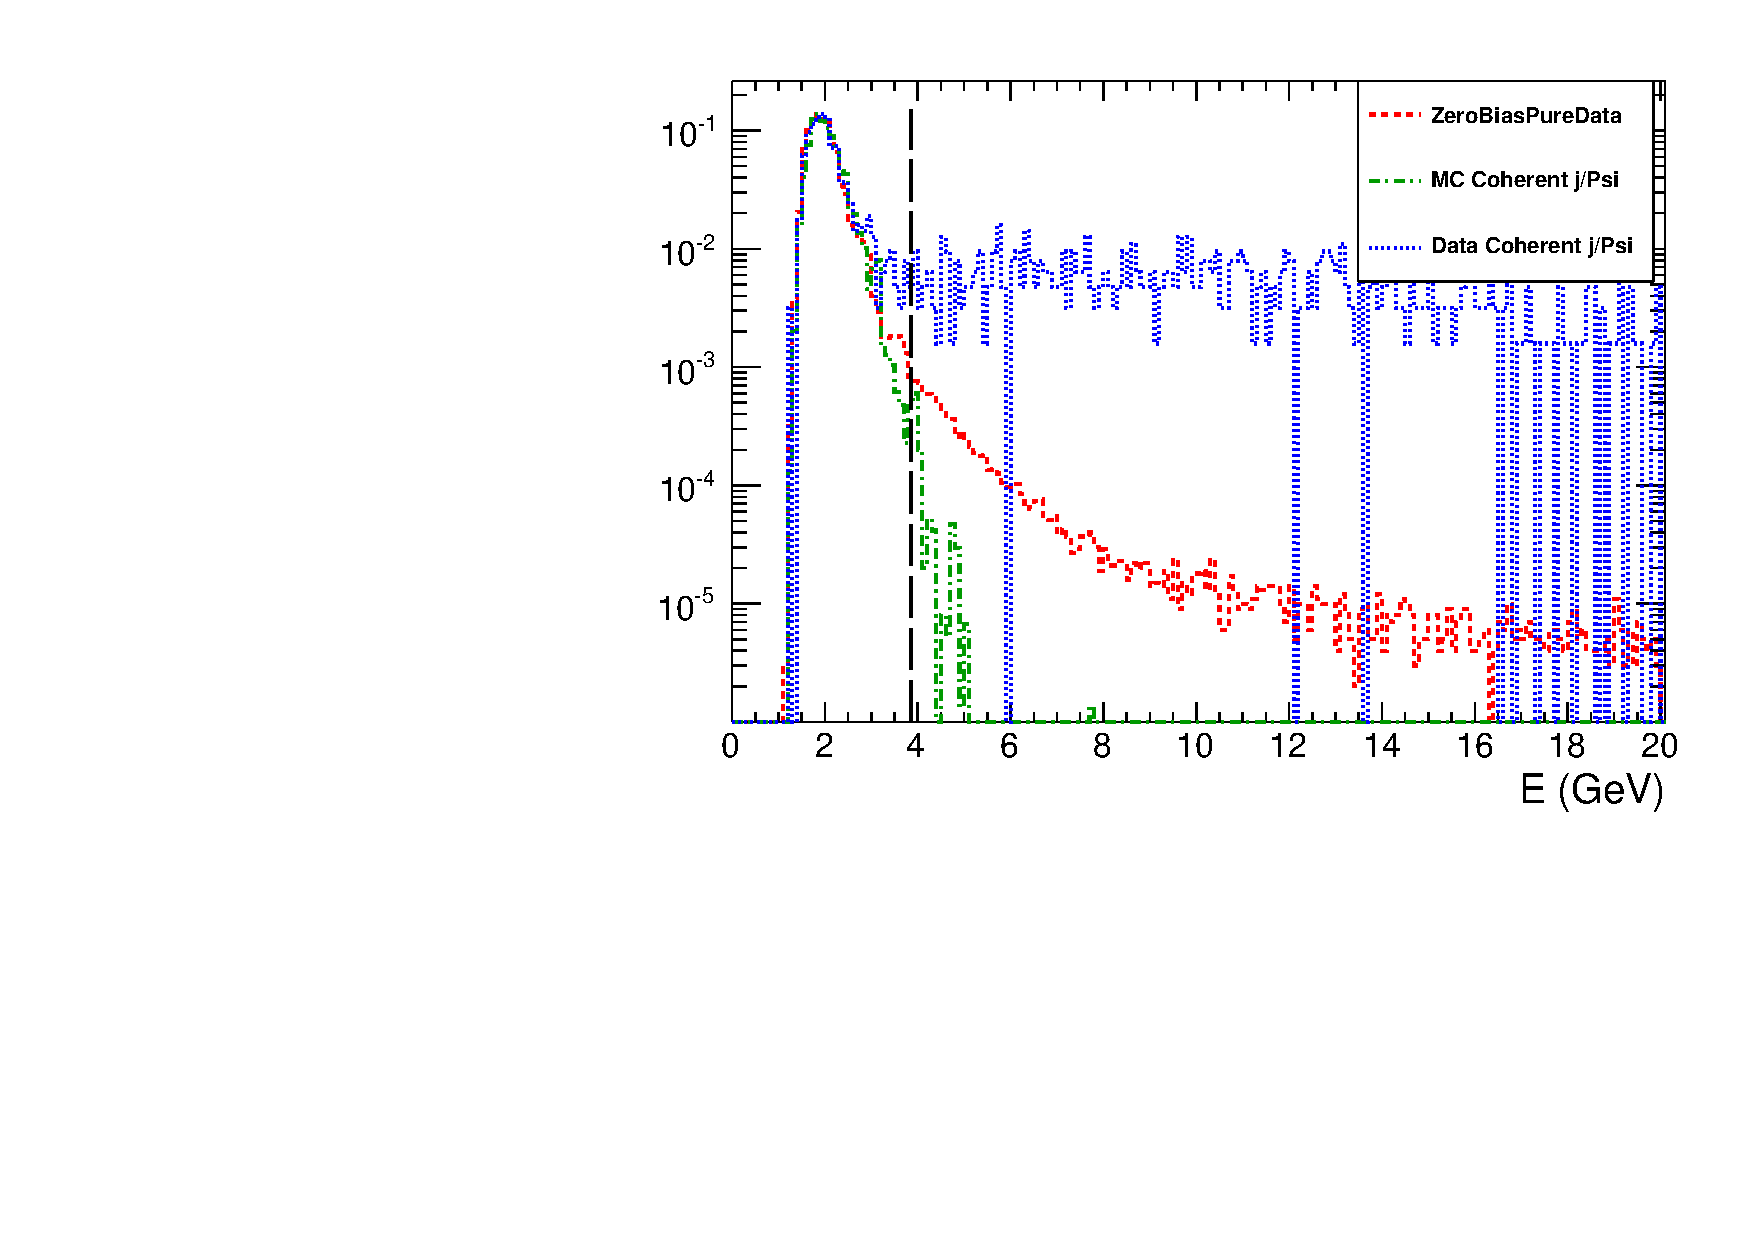
\includegraphics[width=.6\textwidth]{hfNoiseComp}
        \caption{Comparison of HF noise distributions in zero bias data, 
          physics triggered data, and MC.}
        \label{fig:hfNoiseDist}
      \end{figure}

      The following standard muon quality cuts are applied:
      \begin{itemize}
        \item Tracker track matched with at least one muon segment 
          (in any station) in both X and Y coordinates (< 3 $\sigma$).
        \item Cut on number of tracker layers with hits $>$ 5.
        \item Number of pixel layers $>$ 0.
        \item The $\chi^{2}$ per degrees of freedom of the track fit $<$ 3. 
        \item Loose transverse and longitudinal impact parameter cuts, within 3 
          cm in the transverse direction and within 30 cm in the longitudinal 
          direction with respect to the primary vertex.
      \end{itemize}
      These cuts are applied to reduce the number of fake muons and have been 
        validated for other muon analyses \cite{cmsJpPP}.

  \section{\label{sec:sigEx} Signal extraction}
    After all event selection cuts, the remaining events contain a combination 
      of coherent \JPsi{}, incoherent \JPsi{}, and dimuons from the 
      photon-photon process.
    Each process must be separated from the final mix.
    To achieve this, the invariant mass and \pt{} distributions are used 
      to distinguish between the three processes. 
    The photon-photon process is extended in invariant mass whereas the 
      \JPsi{} is peaked strongly near 3.1 GeV.
    The dimuon transverse momentum distribution of the photon-photon and 
      the coherent process have similar distributions, both are sharply peaked 
        below 0.1 GeV, whereas the incoherent process is more broadly 
        distributed across an interval extending to nearly 1 GeV.
    The mass distribution was fit to separate the photon-photon process from
      the \JPsi{} process.
    The \pt{} distribution was used to separate the incoherent process from 
      the photon-photon process, and the coherent process. 
    In this way, a separate yield was extracted for all three processes. 
    
    The invariant mass distribution for opposite sign dimuons is shown in 
      Fig.~\ref{fig:massFit}. 
    A \JPsi{} signal is clearly visible together with tails at higher and
      lower mass due to the photon-photon process.
    A fit to the invariant mass distribution was performed using a Gaussian
      to account for the \JPsi{} signal and a first-order polynomial function 
      for the photon-photon process.
    The extracted number of \JPsi{} candidates from this fit includes all 
      \JPsi{}s in the mass window that passed the analysis cuts, i.e. both
      coherent and incoherent process contribute to yield from the mass
      fit.
    The \pt{} distribution is needed to separate the two different 
      contributions to the \JPsi{} peak. 

    \begin{figure}[!Hhtb]
      \centering
      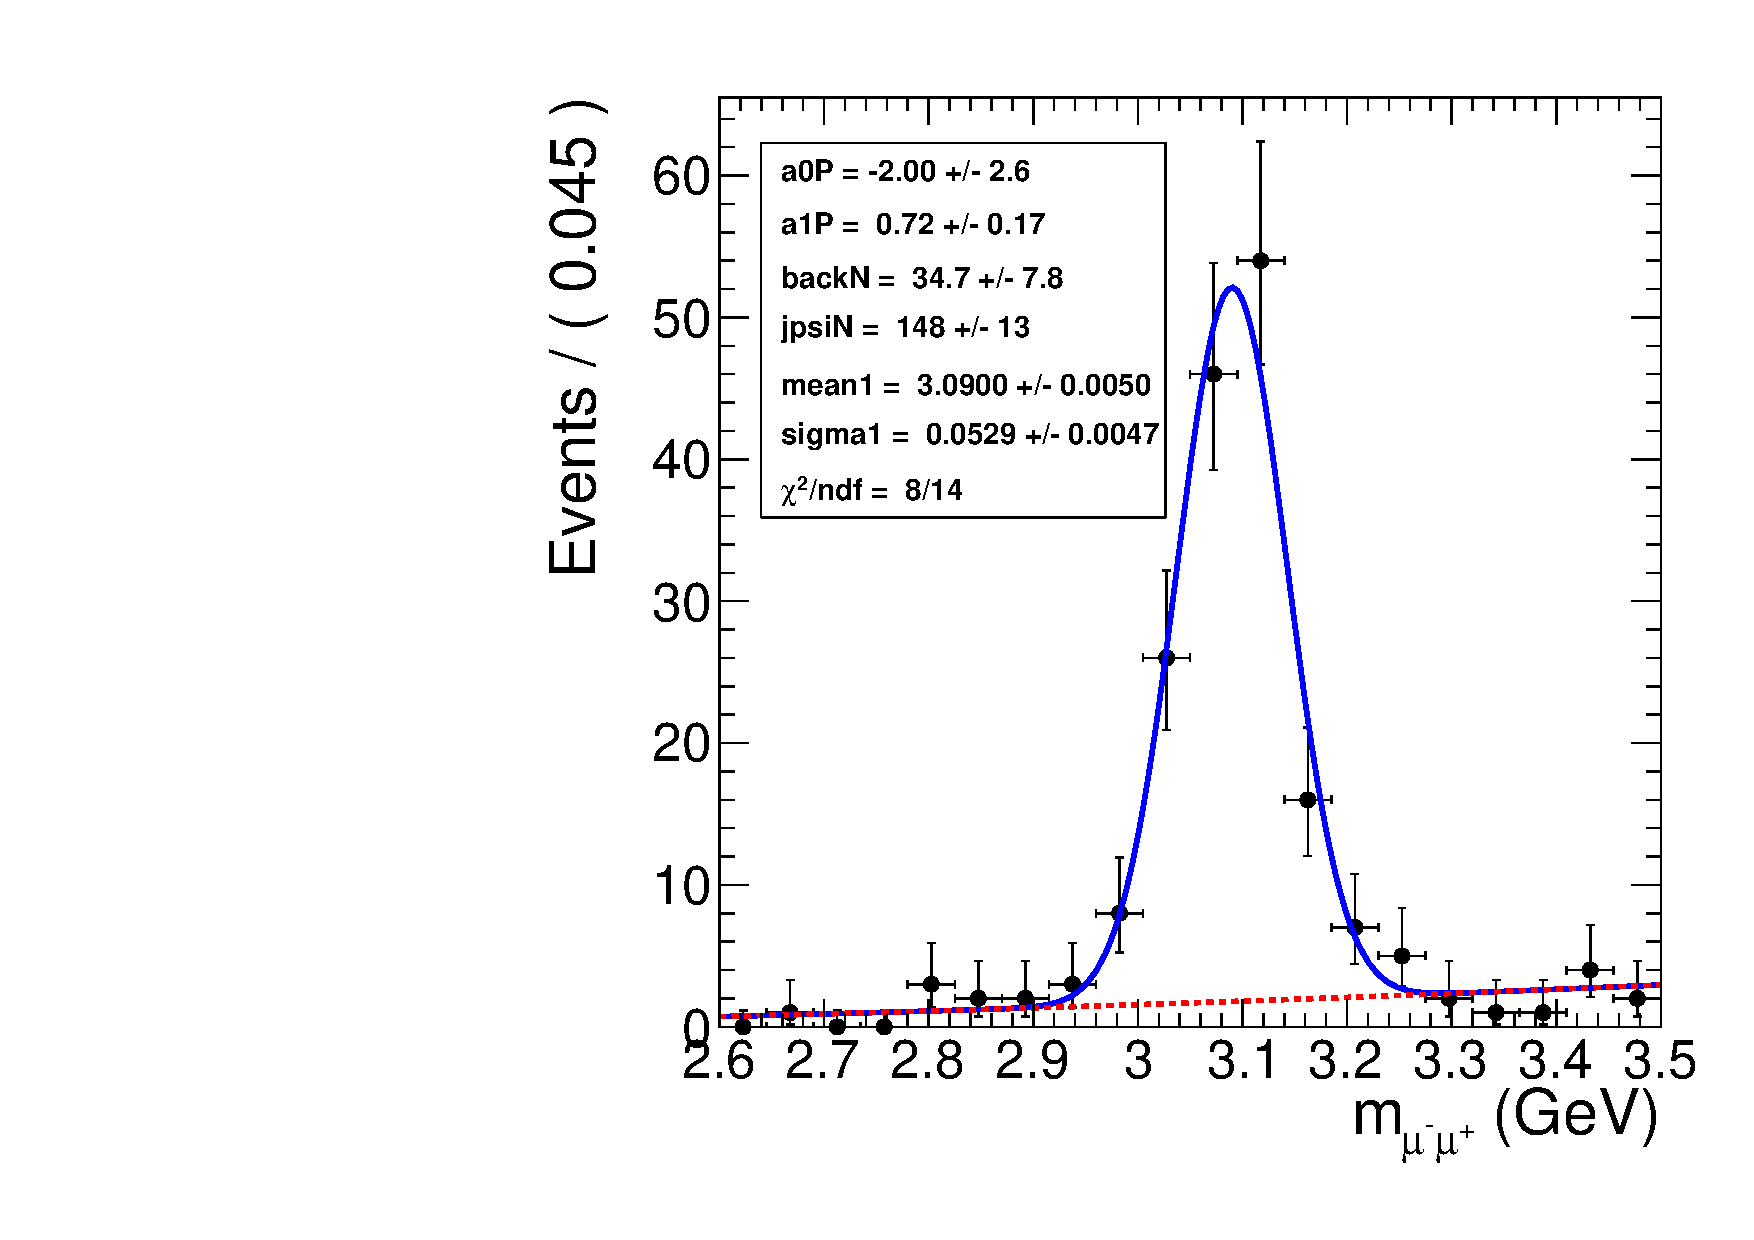
\includegraphics[width=.6\textwidth]{massFitSimple}
      \caption{Mass fit to \JPsi{} using Gaussian for the 
        signal and a first-order polynomial for the photon-photon continuum.}
      \label{fig:massFit}
    \end{figure}
  
    Figure~\ref{fig:ptTemps} shows the \pt{} spectrum of the events plotted 
      in Fig.~\ref{fig:massFit}.  
    There is a clear coherent peak at \pt{} = 60 MeV followed by a broad 
      distribution that with a mean near \pt{} = 450 MeV. 
    To extract the contribution of coherent, incoherent and gamma-gamma 
      processes in the data the spectrum in  Fig.~\ref{fig:ptTemps} was fit to 
      the sum of three MC templates corresponding to the final output of the MC
      simulations for these three processes.       
    The clear overlap of the coherent and photon-photon process, and the 
      clear separation of these two lower \pt{} processes from the incoherent
      process is apparent.
    The shape of the \pt{} distribution for the coherent, incoherent, and 
      photon-photon process are taken from the final output of MC after
      applying all analysis cuts. 
    In Fig.\ref{fig:ptTemps}, the yield parameters that were fit were left
      unconstrained for all three process.

    \begin{figure}[!Hhbt]
      \centering
      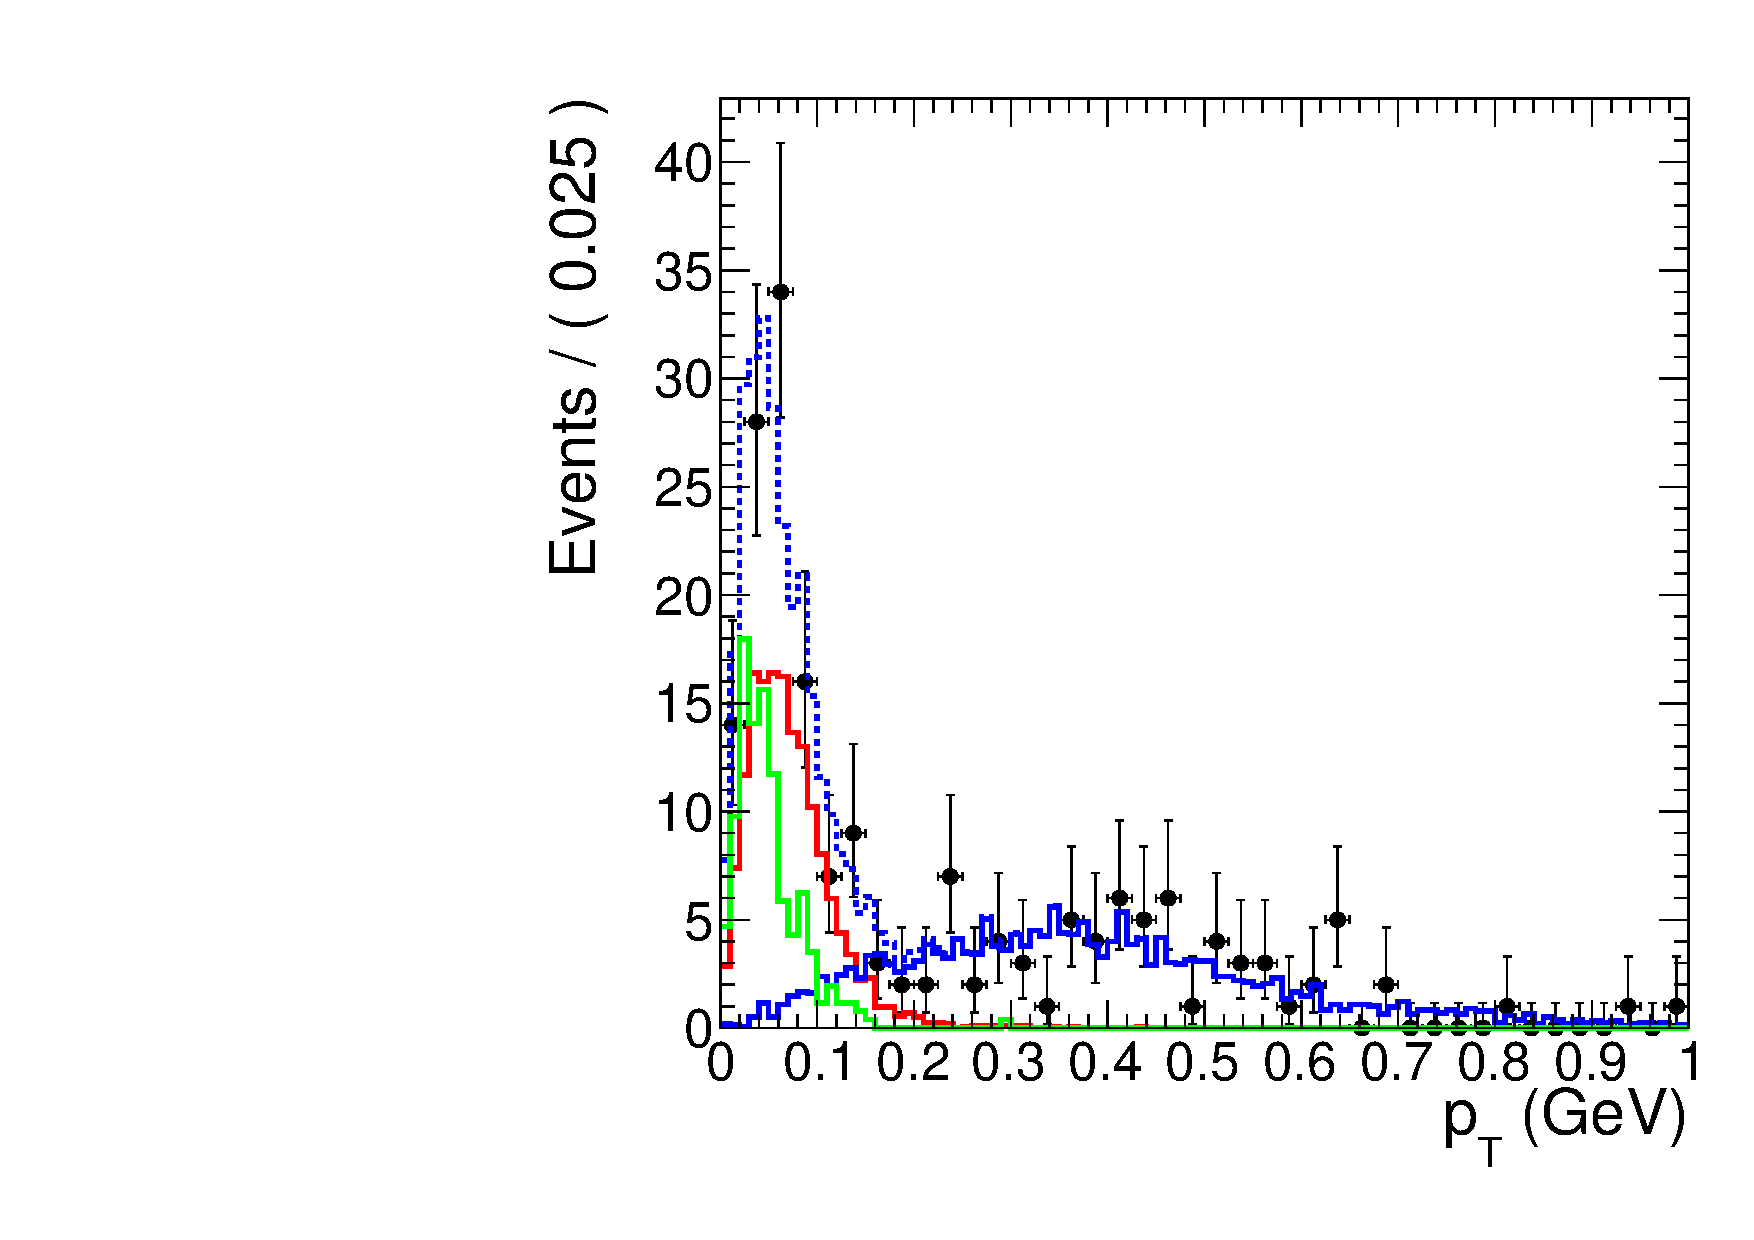
\includegraphics[width=.6\textwidth]{gaussCC}
      \caption{ Fit to MC \pt{} templates. }
      \label{fig:ptTemps}
    \end{figure}

    The shape of the photon-photon and coherent \JPsi{} process are very 
      similar in transverse momentum.
    Accordingly, the contribution from the photon-photon process and the 
      coherent process are difficult to separate from the \pt{} distribution.
    The confidence contours in Fig.~\ref{fig:ptOnlyCor} from the template fit
      in Fig.~\ref{fig:ptTemps} demonstrate the strong anti-correlation 
      between the coherent yield parameter, $nCo$, and the yield parameter 
      for the photon-photon process, $nGamma$.
    Because of the anti-correlation, the statistical uncertainty on $nCo$ and 
      $nGamma$ from the fit are larger than $\sqrt{nCo}$ and $\sqrt{nGamma}$
      expected from Poisson statistics. 
    The information from the invariant mass and \pt{} distributions were
      combined to break this correlation. 
    Through this combination, the contribution to the final yield from 
      the three process was measured.

    \begin{figure}[!Hhbt]
      \centering
      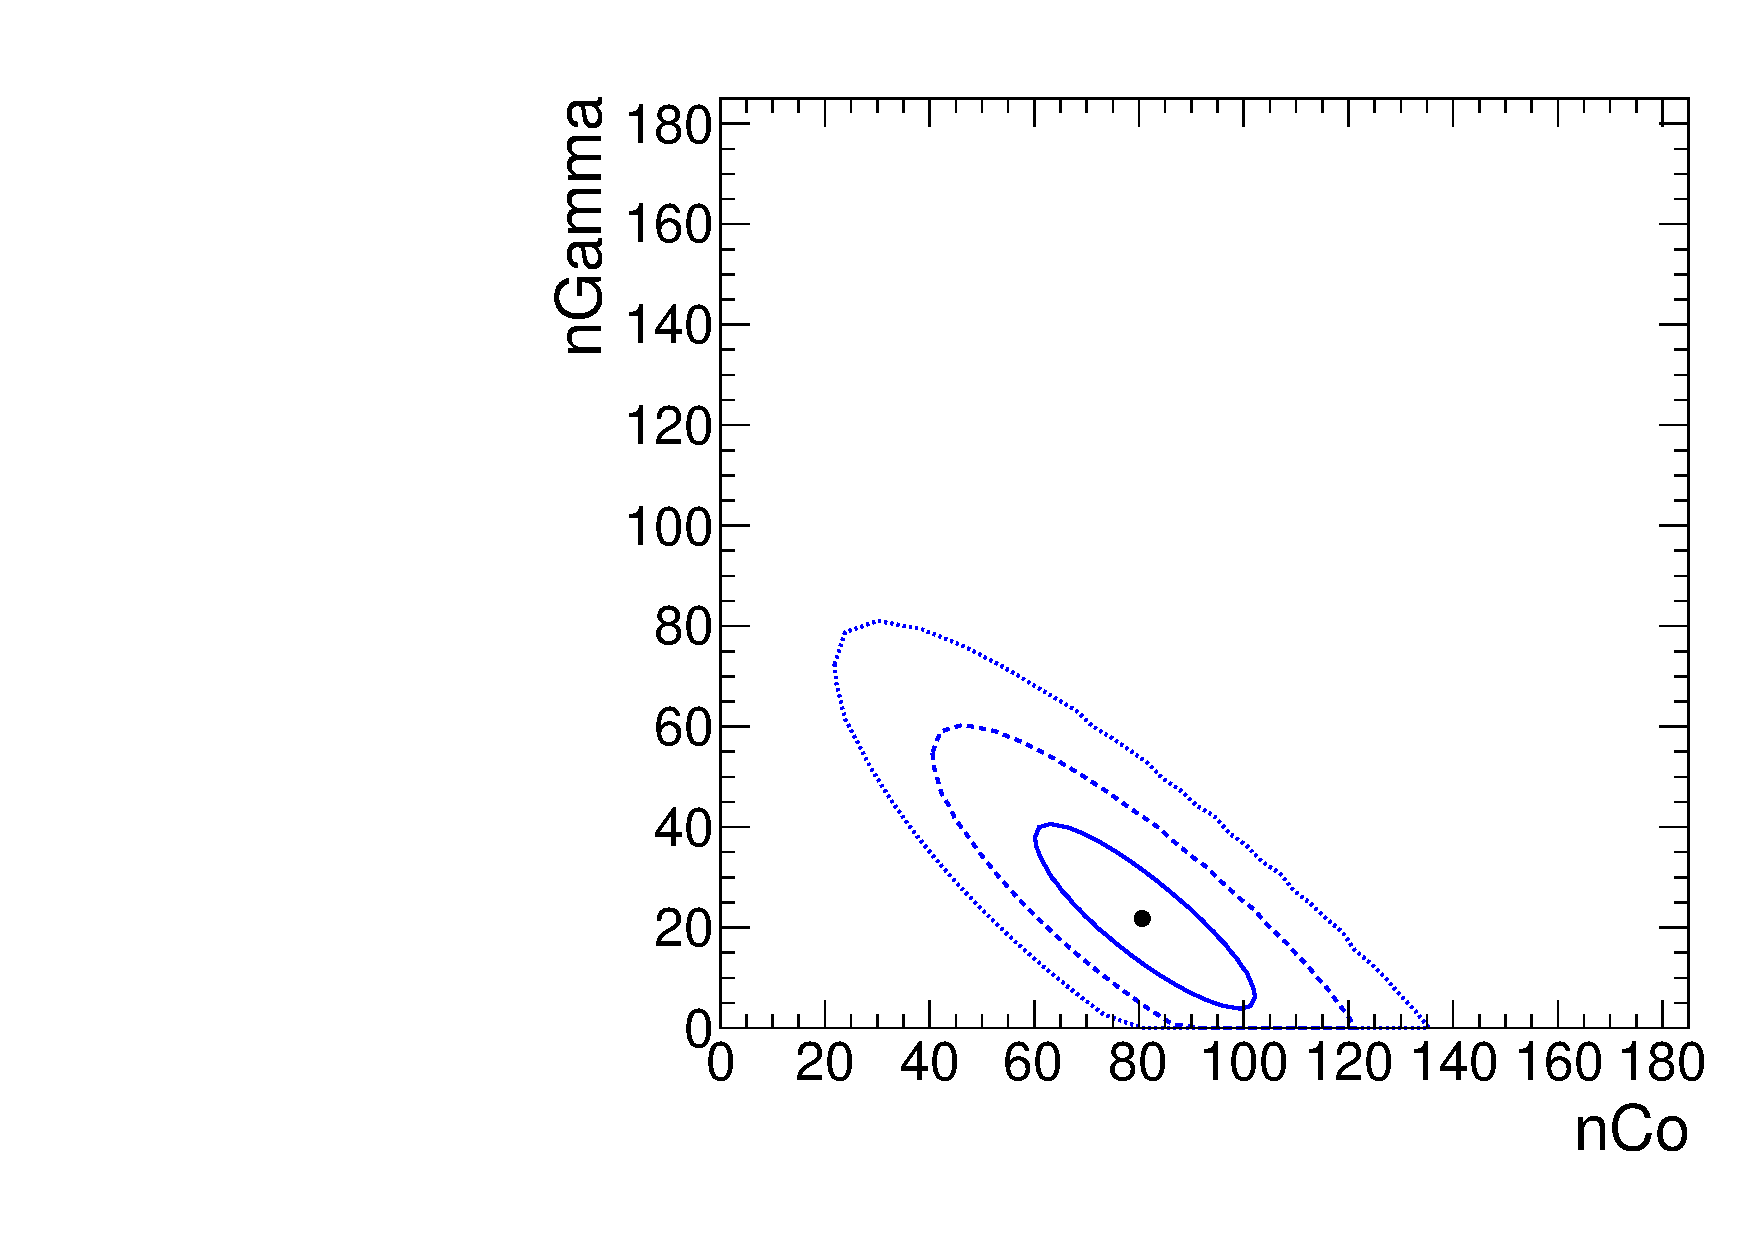
\includegraphics[width=.6\textwidth]{nCoNGammaCorPtOnly}
      \caption{68\%, 95\%, and 99\% confidence contours from the \pt{} 
        template fit. }
      \label{fig:ptOnlyCor}
    \end{figure}

    A simultaneous fit to the mass spectrum and \pt{} 
      spectrum was preformed to utilize the mass fits ability to distinguish 
      the photon-photon process from the coherent and incoherent process all 
      while utilizing the \pt{} fits ability to separate the coherent and 
      photon-photon processes from the incoherent.
    Fig.~\ref{fig:simFitMassPtGauss} shows the result of the simultaneous fit.
    The simultaneous fit forces the parameter $nGamma$ to both describe the 
      photon-photon continuum present in the side bands of the \JPsi{} mass 
      peak as well the photon-photon contribution to the low-\pt{} part of 
      the \pt{} spectrum.
    In addition, the \JPsi{} yield from the mass fit is forced to equal the
      contribution from the incoherent and coherent process in the 
      fit to the \pt{} distribution. 
    In this way, the correlation between the yield parameters was broken, and 
      the contribution from the three process were made independent of each 
      other.
      
    \begin{figure}[!Hhbt]
      \centering
      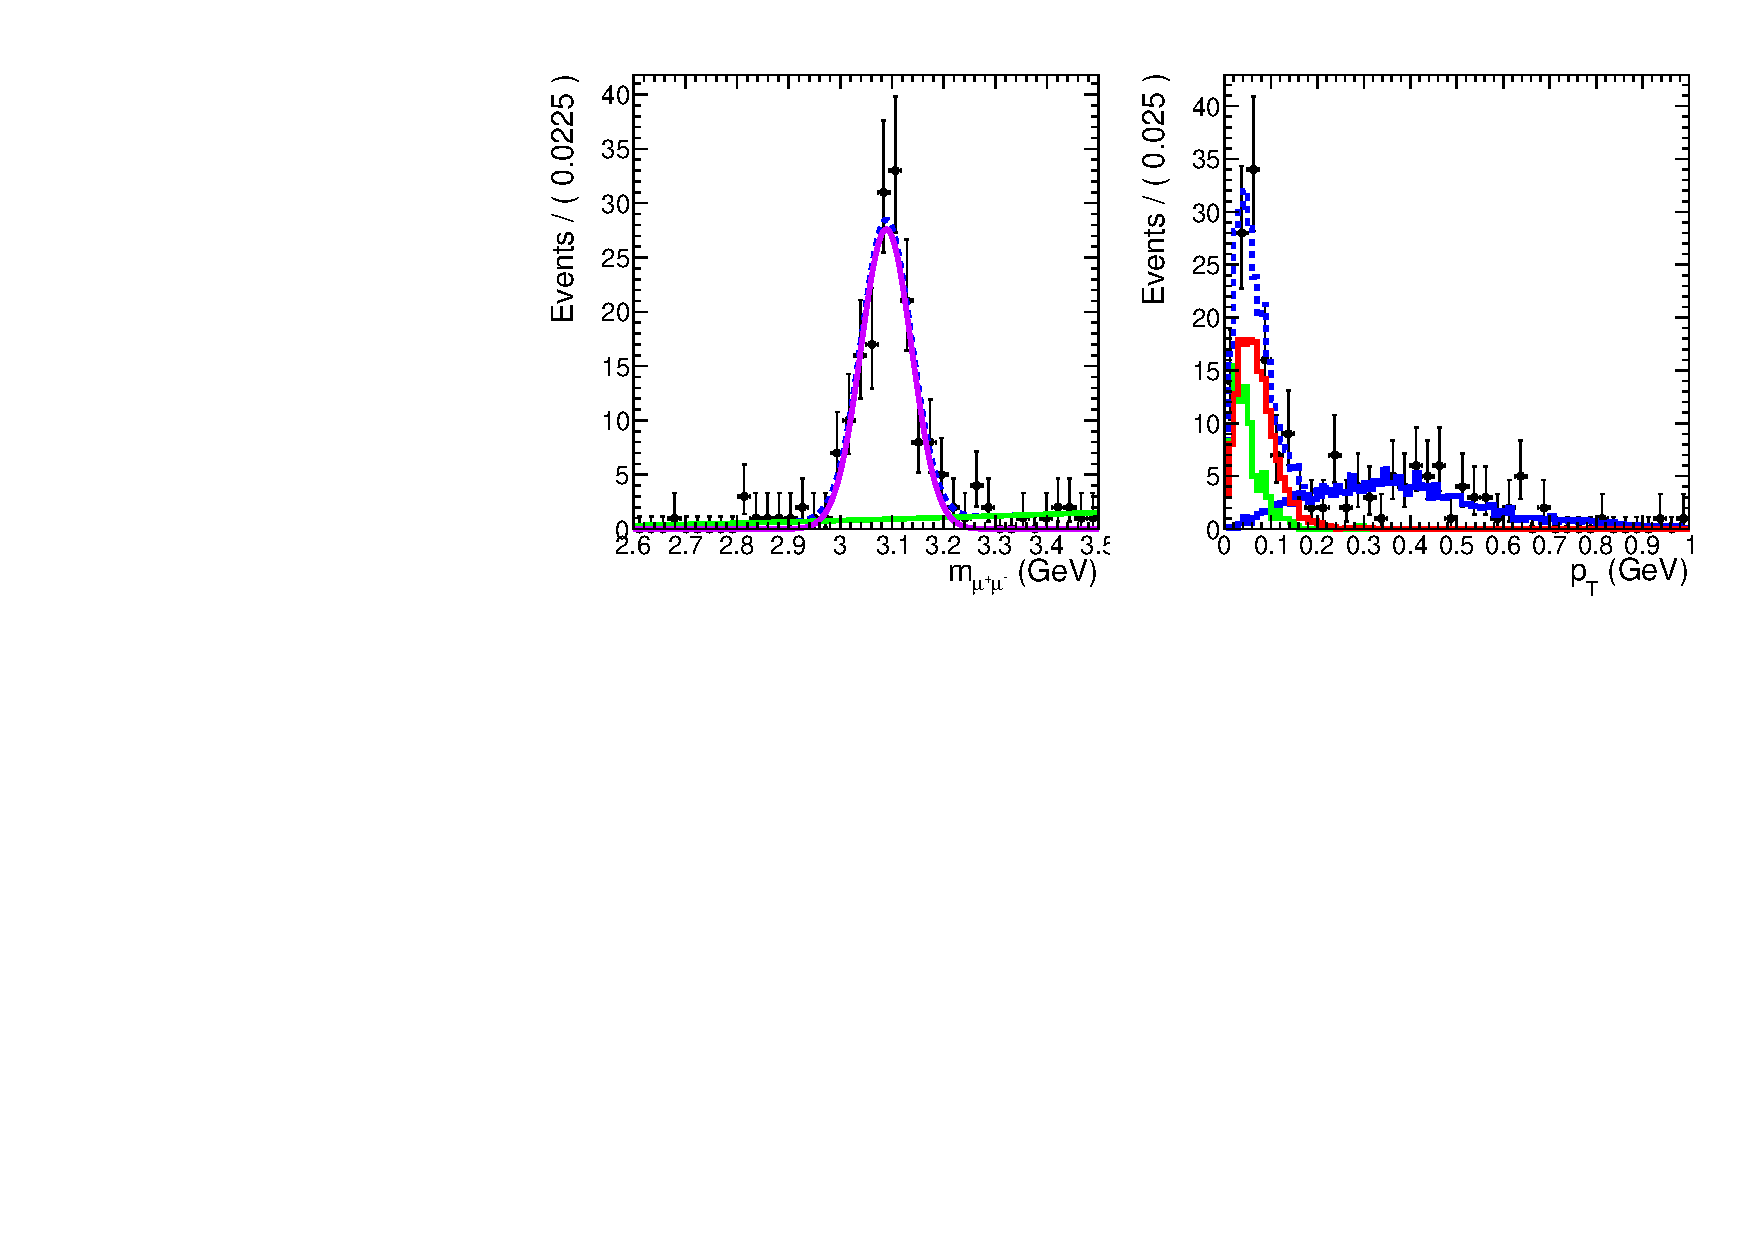
\includegraphics[width=0.9\textwidth]{ptMassSimGaussLine}
      \caption{Simultaneous fit to the mass and \pt{} spectra.}
      \label{fig:simFitMassPtGauss}
    \end{figure}

    Fig.~\ref{fig:simGaussCor} shows the confidence contours for $nCo$ and 
      $nGamma$ from the simultaneous fit in Fig.~\ref{fig:simFitMassPtGauss}.  
    The slope of the confidence contours in Fig.~\ref{fig:simGaussCor} 
      is noticeably than in Fig.~\ref{fig:ptOnlyCor}.
    The contours for the simultaneous fit are also reduced compared to 
      Fig.~\ref{fig:ptOnlyCor} with widths in $nCo$ and $nGamma$ similar to 
      those expected from Poison statistics. 
    From the simultaneous fit, reasonable statistical errors were obtained 
      along with the yields for the three processes. 

    \begin{figure}[!Hhbt]
      \centering
      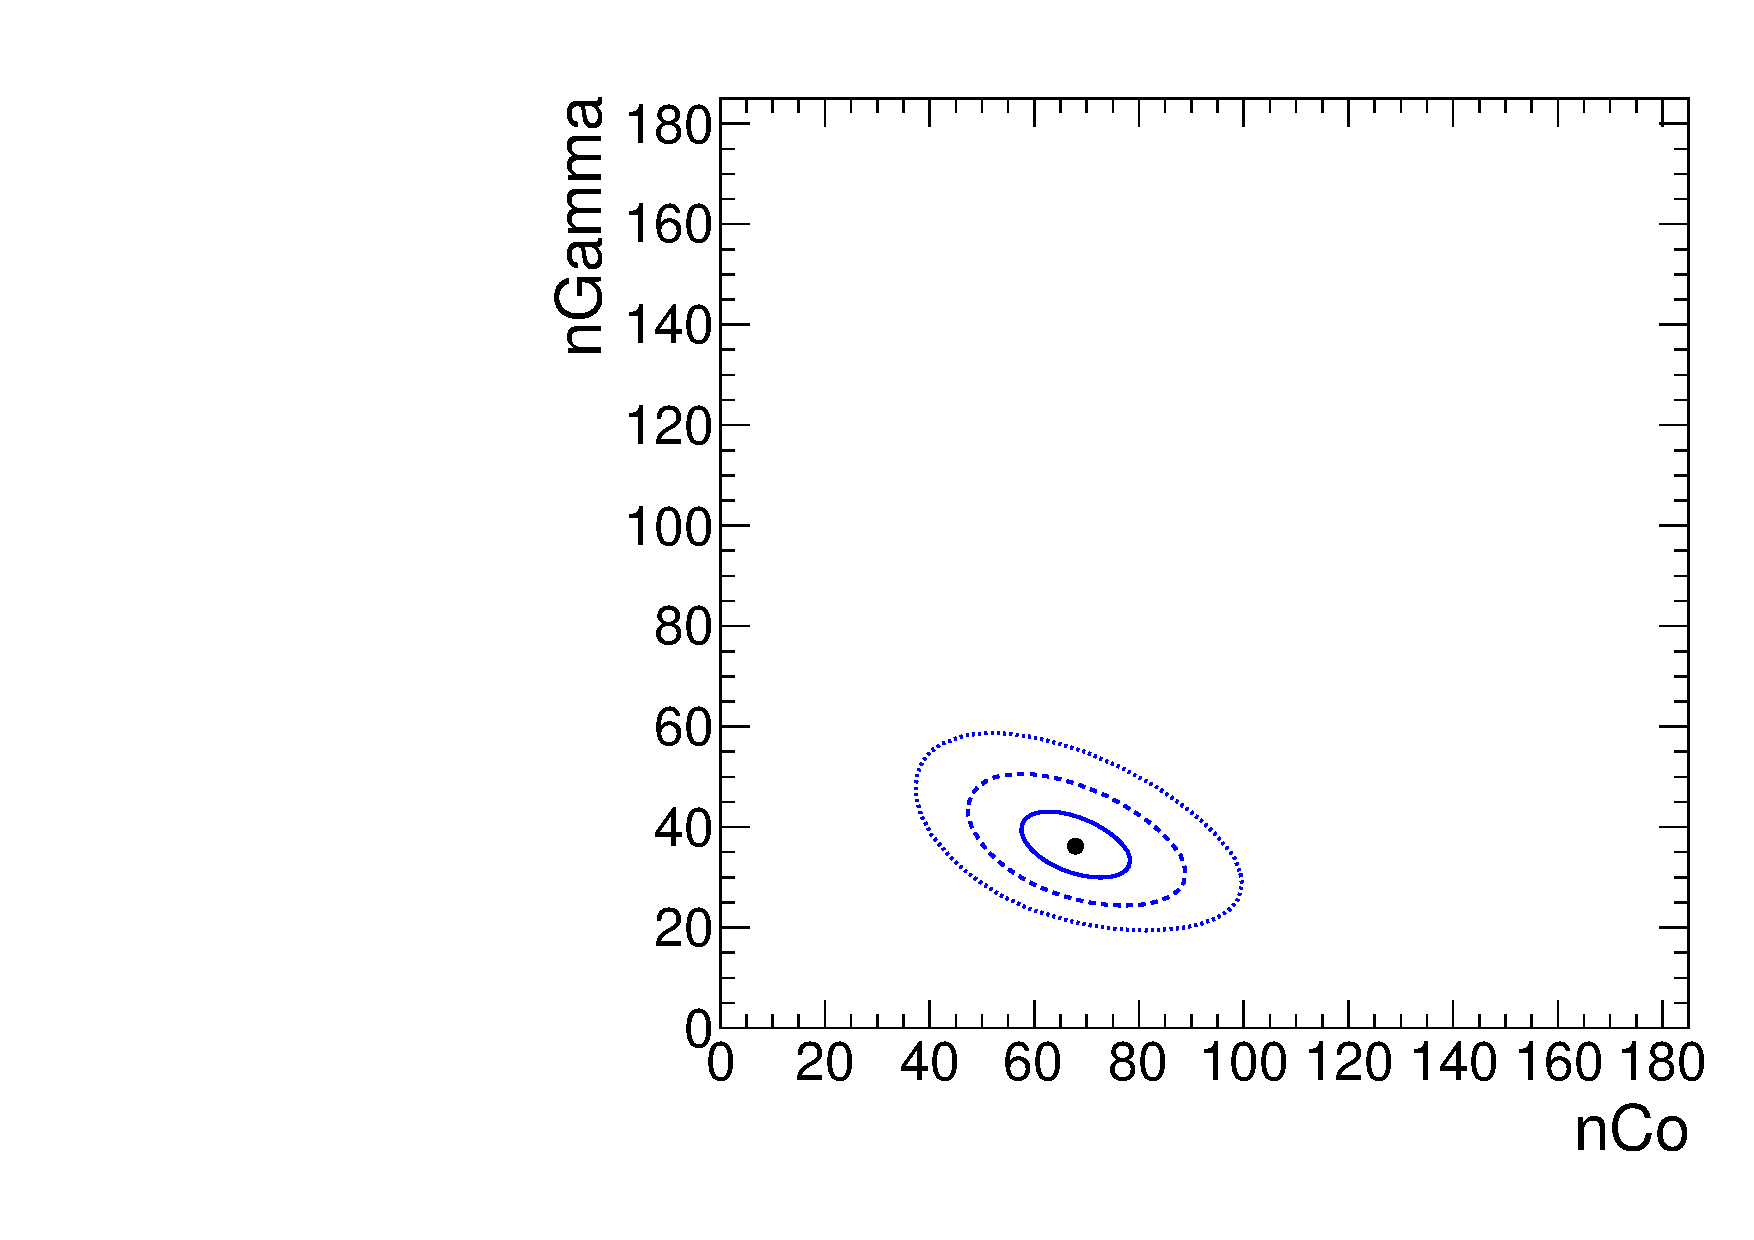
\includegraphics[width=0.6\textwidth]{nCoNGammaCorPtMass}
      \caption{68\%, 95\%, and 99\% confidence contours from the 
        simultaneous fit. }
      \label{fig:simGaussCor}
    \end{figure}

  \section{\label{sec:effDet} Efficiency determination}
    Each step of the triggering, event selection, and analysis has an associated
      efficiency that must be accounted for in the  measurement of the \JPsi{} 
      cross section.  
    The ZDC trigger efficiency, the muon trigger efficiency, and the muon 
      reconstruction efficiency are the two most significant contributors to 
      the total efficiency measurement. 
    The efficiency of the pixel track requirement, and the veto on activity in 
      the BSCs from the trigger are also estimated but found to be consistent 
      with fully efficient. 
    The following section explains how each of these efficiencies was measured
      with a special emphasis on the ZDC trigger efficiency and the muon 
      trigger and reconstruction efficiencies. 

    \subsection{Muon efficiencies}
      The muon efficiencies were measured using a combination of MC and data 
        based methods.
      The MC based measurement accounts for the detector acceptance and the 
        efficiency of the muon quality cuts discussed in 
        Section~\ref{sec:DataSetEvSel}.
      The trigger efficiencies were measured in data using the tag and probe 
      method \cite{cmsTnP}, which is discussed below. 

      CMS has a limited acceptance for \JPsi{}s, particularly in the case of 
        \JPsi{}s with low momentum like those produced in UPC events. 
      To measure the acceptance of CMS for \JPsi{}s, reconstructed dimuon 
        candidates were considered detectable if both reconstructed muon 
        daughters fell into a detectability region in \pt{} and $\eta$.
      The muon detectability region was defined using the coherent \JPsi{} 
        events obtained from STARlight.
      The efficiency for reconstructing single muons $\varepsilon^{\mu}_{reco}$ 
        is defined by $\varepsilon^{\mu}_{reco} = \frac{N^{\mu}_{reco}}{N^{\mu}_{gen}}$, 
        where $N^{\mu}_{reco}$ is the number reconstructed muons obtained 
        after the full CMS detector simulation that passed the standard
        muon quality cuts, and $N^{\mu}_{gen}$ is the number of generated 
        muons from STARlight.
      \begin{figure}[!Hhtb]
        \centering
          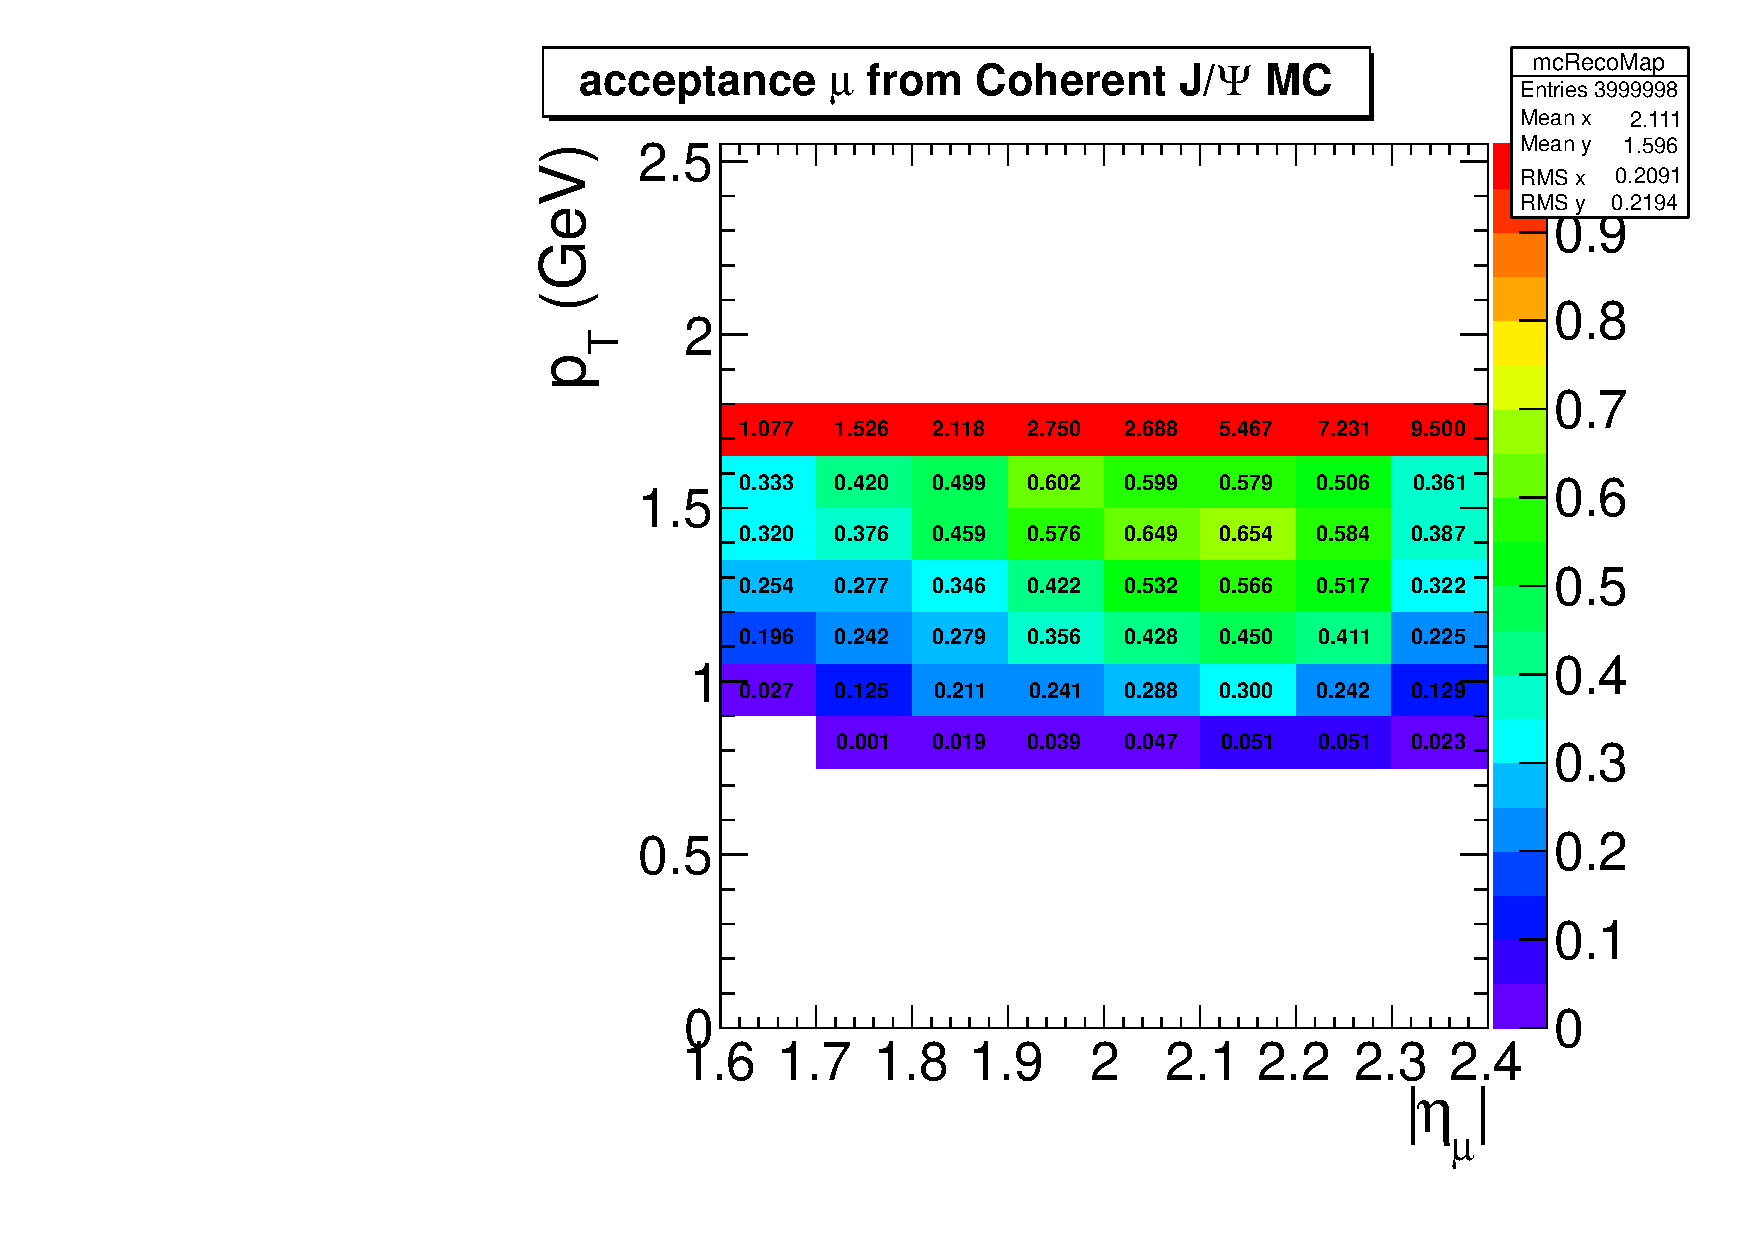
\includegraphics[width=.6\textwidth]{mcEffMaps/accMuJpCo} 
        \caption{ Muon daughter detectability from coherent \JPsi{}}
        \label{fig:muonDaughterDet}
      \end{figure}
      Fig.~\ref{fig:muonDaughterDet} shows the efficiency for reconstructing
        single muons from coherent \JPsi{} events.
      To avoid the edges of the detectors acceptance, all reconstructed muons 
        that fall into a (\pt{},$|\eta|$) bin that has an efficiency less 
        than 20\% were rejected.
      This condition defines the detectability region.
      The acceptance and reconstruction efficiency for reconstructing dimuons 
        was calculated from MC using the following formula:
      \begin{equation}
        A \times \varepsilon=\frac{N_{det}(|y|)}{N_{gen}(|y|)},
        \label{eq:jpsiAccEq}
      \end{equation}
        where $N_{det}$ is the number of reconstructed dimuons where both 
        daughters fall into the detectability region, and $N_{gen}$ is the
        number of generated dimuons. 
      From Eq.~\ref{eq:jpsiAccEq}, the acceptance for \JPsi{} was calculated
        as a function of $|y|$, and \pt{} (see Fig.~\ref{fig:jpsiAcceptance}).
        \begin{figure}[!Hhtb]
          \centering
            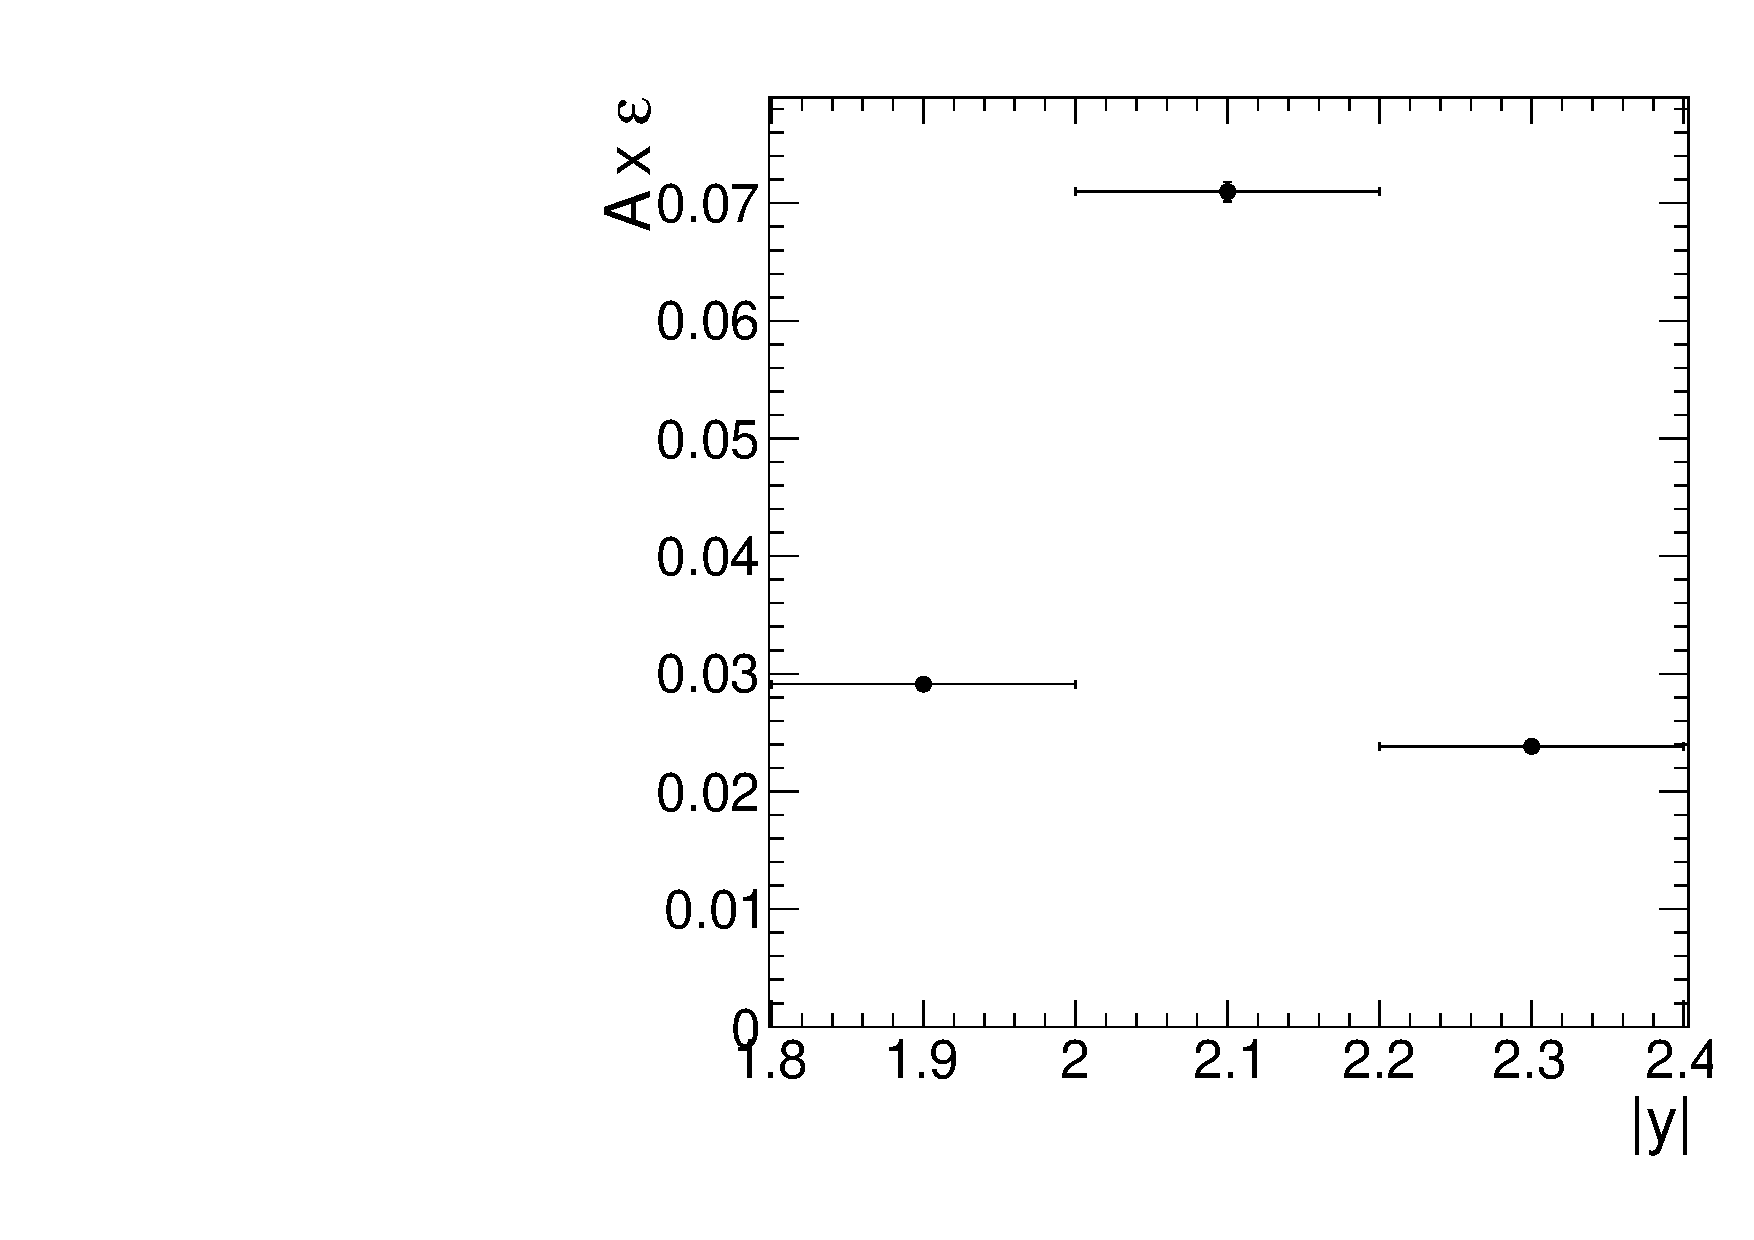
\includegraphics[width=.45\textwidth]{accXeffFromMC1d}
          \caption{Dimuon acceptance from coherent \JPsi{}.}
          \label{fig:jpsiAcceptance}
        \end{figure}

      The ``tag and probe method'' is a data driven approach used to measure the 
        trigger efficiency of the muon daughters from \JPsi{} decays.
      In this method there are three categories of daughter muons. 
      \textit{Tag muons} are high quality muons.
      \textit{Passing probes} are reconstructed muons that match the muon 
        trigger, while \textit{failing probes} do not. 
      Each dimuon will have one daughter classified as a tag and the other
        as a probe.
      From here three invariant mass histograms are studied. 
      One histogram is created from all pairs. 
      The second comes from pairs where the probe is a passing probe.  
      The last histogram comes from pairs where the probe fails to fulfill
        the trigger, it is a failing probe. 
      By matching the tag to the trigger, the probe is unbiased by the trigger 
        and the  efficiency can be measured by fitting the three mass 
        histograms. 

      Because the trigger efficiency depends on the \pt{} and $|\eta|$ of the 
        muon, one set of three histograms for each (\pt{},$|\eta|$) bin of the
        probe is created.
      To extract the single muon trigger efficiency $\varepsilon^{\mu}_{trig}$, 
        each set of invariant mass histograms were simultaneously fit. 
      The signal was fit using a Crystal Ball function \cite{Gaiser:1982yw}, and the background 
        was fit to an exponential.
      The Crystal Ball parameters were simultaneously fit to all three 
        histograms.
      The exponential function was fit to the failing and passing probe 
        histograms separately.
      Because the background shapes are in principle different for the two 
        samples, the efficiency is driven by this difference. 

      Fig.~\ref{fig:tnpFitPlot} shows the fit of the three sets of pairs. 
      \begin{figure}[!Hh]
        \centering
        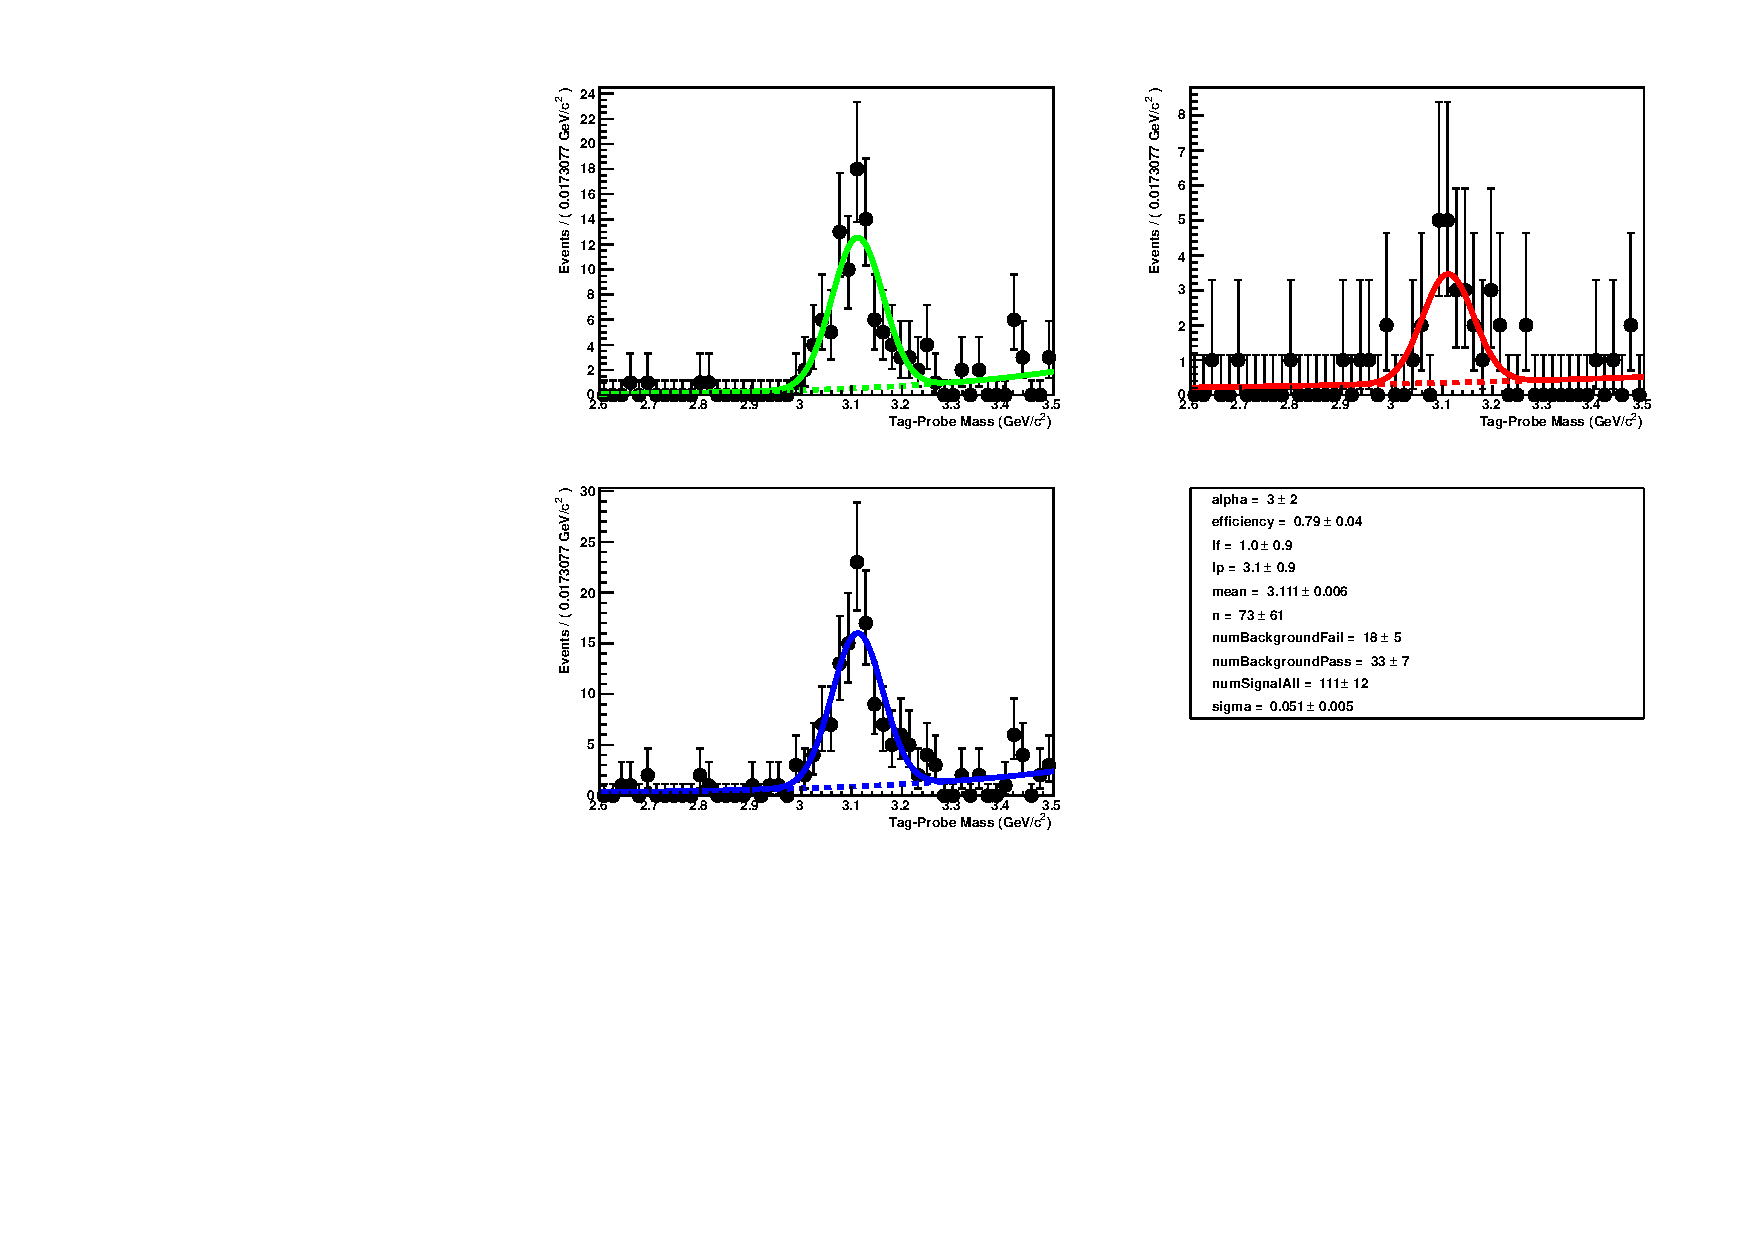
\includegraphics[width=1.0\textwidth]{tNp/tnpFits}
        \caption{Fits to tag and probe pairs in the \JPsi{} mass region for
        pairs with a probe 2 < |$\eta$| < 2.2 and 1.55 < \pt{} < 1.8 GeV.}
        \label{fig:tnpFitPlot}
      \end{figure}
      This fit was done for each bin of the probes \pt{} and $\eta$.
      The efficiency from the fits in each bin are shown in Fig.~\ref{fig:tnpTrigMap}.
      \begin{figure}[!Hhbt]
        \centering
        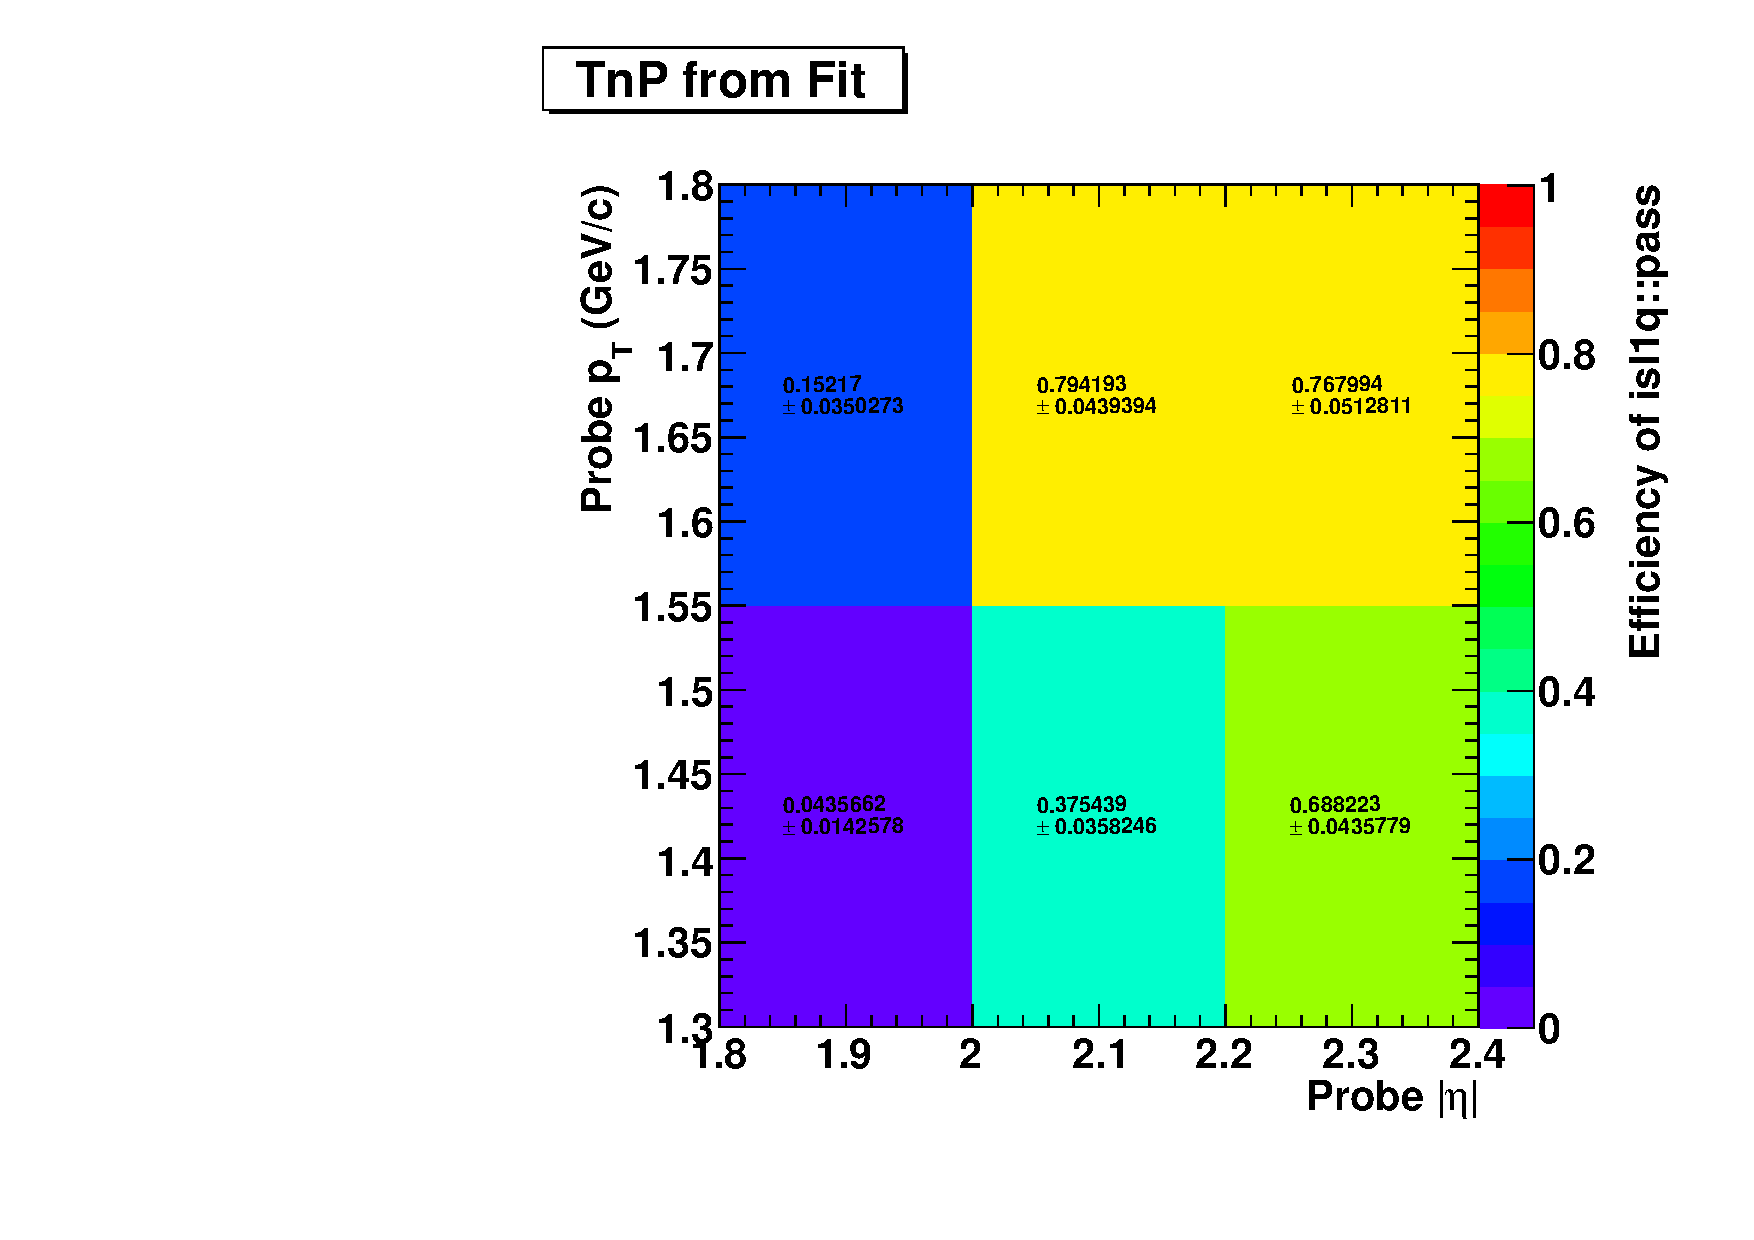
\includegraphics[width=.6\textwidth]{tNp/tnpFromFit}
        \caption{Muon trigger efficiencies in \pt{} and $\eta$ bins from 
          the tag and probe method.}
        \label{fig:tnpTrigMap}
      \end{figure}

      The dimuon trigger efficiency $\varepsilon^{dimuon}_{trigger}$ was 
        calculated from the single muon efficiencies using the following
        equation:
      \begin{equation}
        \label{eq:dimuTrigEff}
        \varepsilon^{dimuon}_{trigger}=1-(1-\varepsilon_{trigger}^{\mu_{1}})(1-\varepsilon_{trigger}^{\mu_{2}}),
      \end{equation}
      where $\varepsilon_{trigger}^{\mu_{1}}$ is the tag and probe efficiency
        of the first dimuon daughter, and $\varepsilon_{trigger}^{\mu_{2}}$ is
        the efficiency of the second muon daughter. 
      In Eq.~\ref{eq:dimuTrigEff} the probability of at least one daughter
        firing the trigger is calculated by subtracting one from the
        probability that neither daughter fires the trigger,
        thus giving the dimuon trigger efficiency. 

      The average dimuon trigger efficiency for each dimuon $|y|$ bin
        was calculated by averaging the efficiency of dimuon candidates in each
        bin. 
      \begin{figure}[!Hhbt]
        \centering
        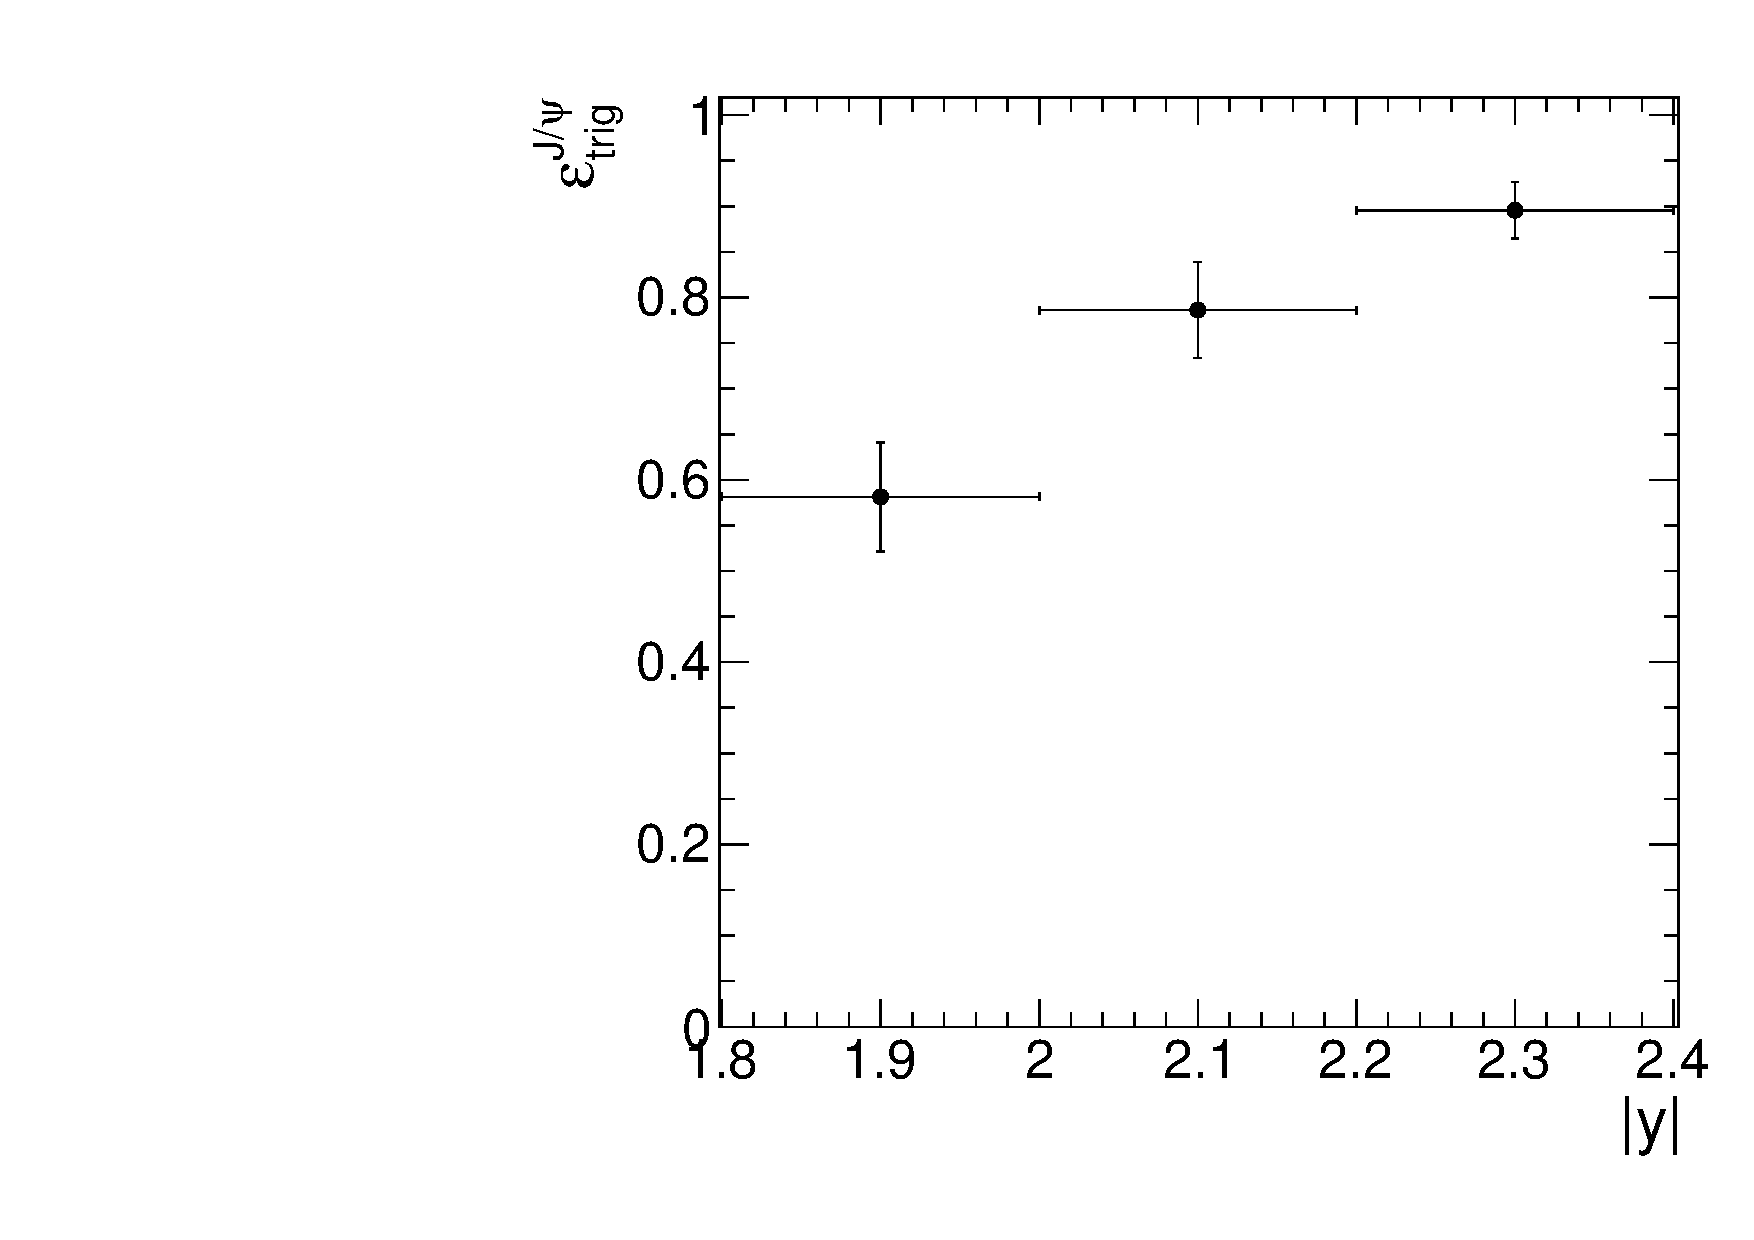
\includegraphics[width=0.6\textwidth]{muTrigEffFromTnP1d}
        \caption{The trigger efficiency from tag and probe averaged over candidates
          in each $|y|$ bin.}
        \label{fig:triggerEffDiMu}
      \end{figure}
      The dimuon trigger efficiency ranges from about 50\% to 90\%. 
      As expected the \JPsi{} trigger efficiency increases with rapidity since 
        the longitudinal momentum of the \JPsi{} is given by 
        $p_Z= M_{J/\psi} \cdot sinh(y)$. 
      Thus \JPsi{} mesons at forward rapidity distribute more momentum to their
        daughter muons which therefore have a greater chance of punching 
        through into the muon chamber.  
      The average trigger efficiency was multiplied by the acceptance and 
        reconstruction efficiency from the MC to produce a total factor for 
        both efficiency and acceptance. 
      \begin{figure}[!Hhtb]
        \centering
        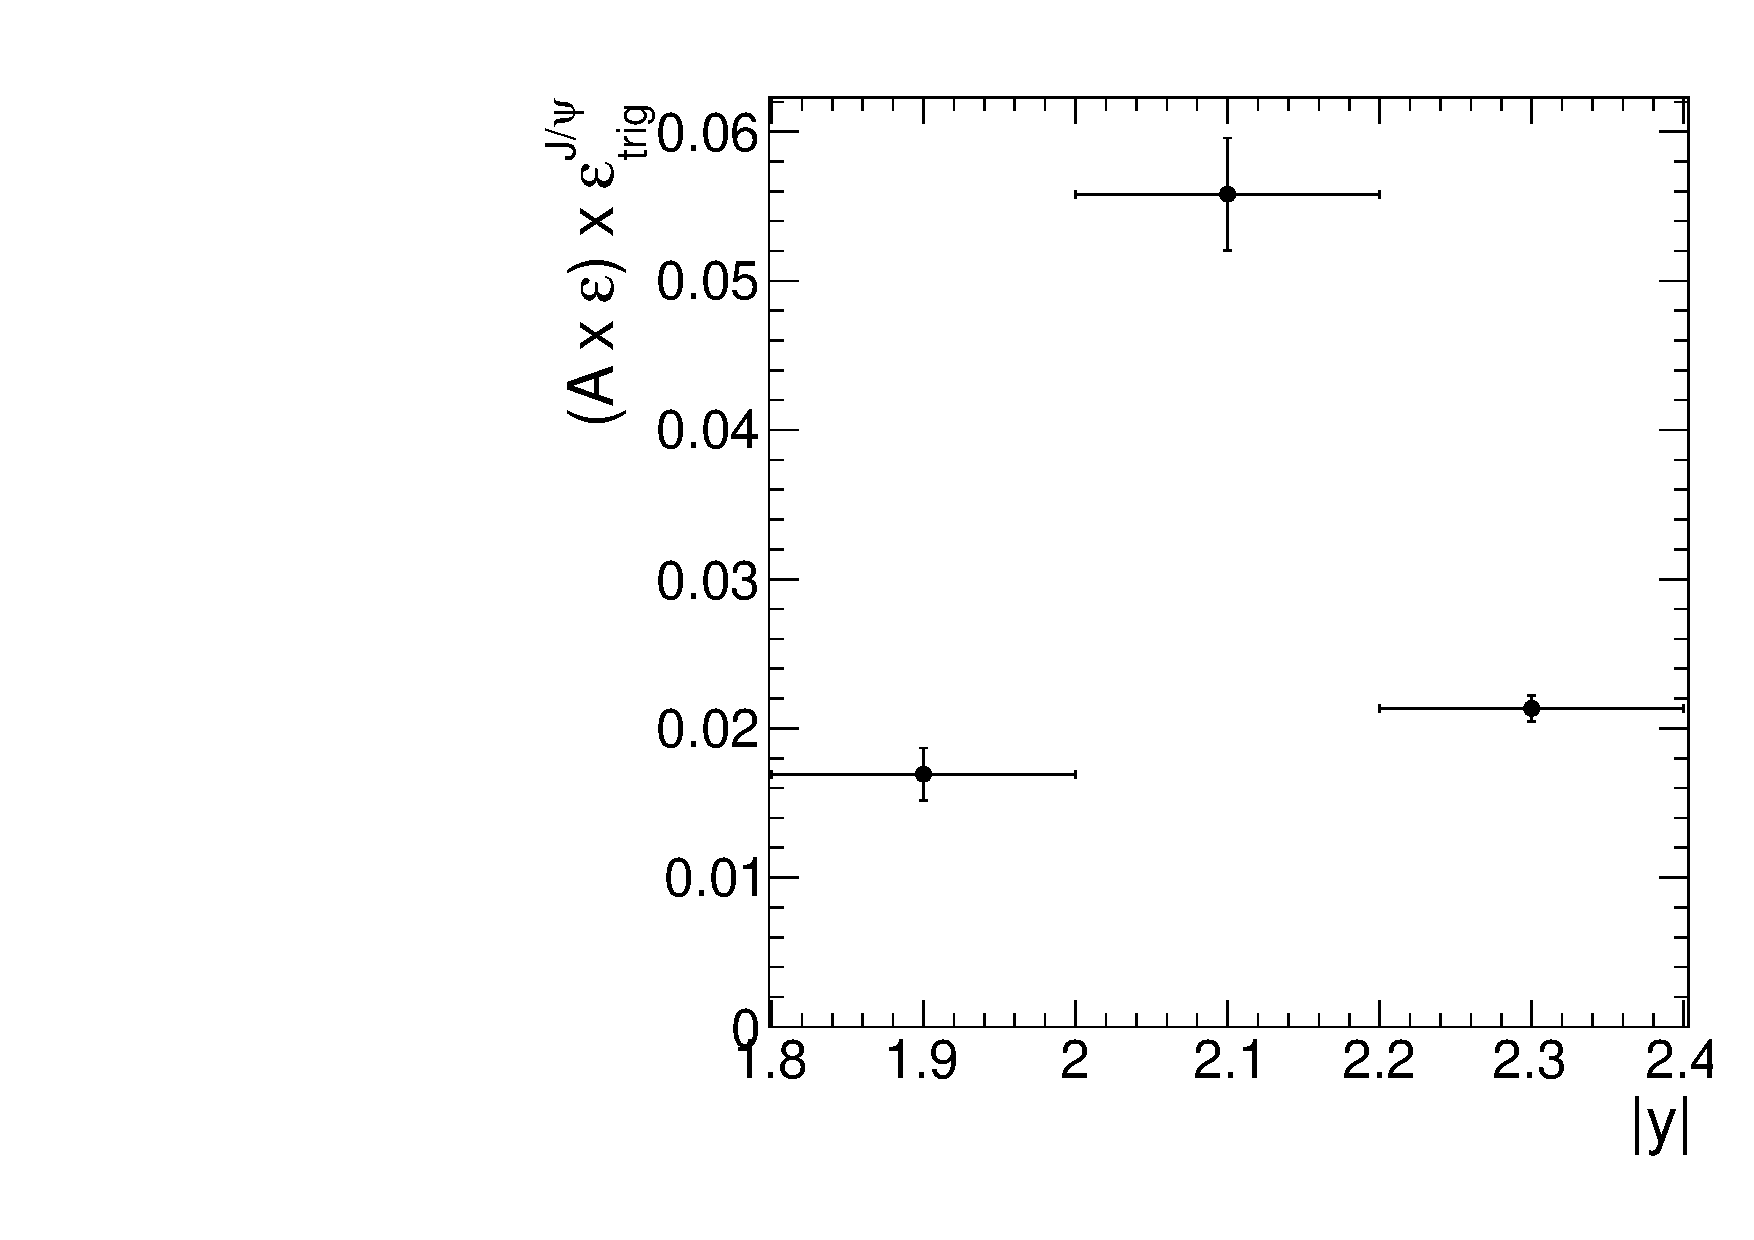
\includegraphics[width=0.6\textwidth]{accXeffTrigg}
        \caption{The acceptance times averaged trigger efficiency from tag and 
          probe.}
        \label{fig:averageExA}
      \end{figure}

      The total combined efficiency and acceptance factor for coherent \JPsi{} 
        between $2.0 \le |y| \le 2.2$ was found to be $\approx 5$\%.
      The acceptance factor of roughly 7\% from the MC was found to be the main
        contributor to the total efficiency. 
      The interplay of the polarization of the \JPsi{} and the material in 
        detector drives down the efficiency by creating an effective momentum 
        threshold for detection (see Section~\ref{sec:mcSim}).
      The reconstruction efficiency of the daughters range between 
        20\%-60\% for muons in the defined detectability range. 
      The trigger efficiency for the detectable muons ranges from 30\%-80\% 
        depending on \pt{}. 

    \subsection{ZDC trigger efficiency}
      As discussed in Section~\ref{sec:breakUpDet}, the trigger labeled 
        ``L1ZDCOr and Pixel Track'' in Table~\ref{tab:hltTriggers2011} was used 
        to measure the ZDC trigger efficiency. 
      This trigger required either a ZDC$^{+}$ or ZDC$^{-}$ trigger, together with at 
        least one pixel track. 
      The veto on the BSC minimum bias trigger, as in the physics triggers, was
        applied offline.
      The BSC veto excludes events where BSCs from both sides of the 
        interaction point are above threshold. 
      This trigger was used in order to collect the most inclusive possible 
        sample without using the minimum bias triggers designed to collect 
        hadronic interactions.
        
      This ZDC triggered sample suffers from a trigger bias. 
      For example, a sample triggered by ZDC$^{+}$ would always produce a 
        ZDC$^{+}$ trigger efficiency of one. 
      To avoid this, a similar technique to tag and probe was used.
      Each event is either tagged as triggered by ZDC$^{+}$ or triggered 
        by the ZDC$^{-}$. 
      The ZDC$^{+}$ trigger efficiency is measured from the ZDC$^{-}$ tagged 
        sample, and vice versa.

      To estimate the efficiency, the number of events with energy in 
        ZDC$^{+}$ greater than the single neutron threshold, N$_{events}$, 
        was measured.
      From this set of events, the number of events that also fire the 
        ZDC$^{+}$, N$_{trig}$, was measured.
      The ratio between the number of single neutron events that fired the 
        trigger and all single neutron events was taken as the estimate of 
        trigger efficiency. 
      The same procedure was applied for each side of the ZDC.
      The trigger efficiency was found to be 98\% for ZDC$^{-}$
        and 94\% for ZDC$^{+}$.
      \begin{table}
        \centering
        \begin{tabular}{|c|c|c|c|c|}
           \hline ZDC Side & N$_{events}$ & N$_{trig}$ & $\varepsilon_{ZDC}$ \\ \hline
           ZDC$^{-}$ & 73028  & 71706  & 0.9819  $\pm$ 0.0037 \\ \hline
           ZDC$^{+}$ & 76132  & 71859  & 0.9439  $\pm$ 0.0035 \\ \hline
        \end{tabular}
        \caption{ZDC trigger efficiencies for ZDC reconstruction method 1 and 
          2}
        \label{tab:zdcEfficiency}
      \end{table}
